\documentclass{rlreport}
\usepackage{listings}
\usepackage{xcolor}

% Custom colors for Python syntax highlighting
\definecolor{codegreen}{rgb}{0,0.6,0}
\definecolor{codegray}{rgb}{0.5,0.5,0.5}
\definecolor{codepurple}{rgb}{0.58,0,0.82}
\definecolor{backcolour}{rgb}{0.95,0.95,0.92}

\lstdefinestyle{mystyle}{
    backgroundcolor=\color{backcolour},
    commentstyle=\color{codegreen},
    keywordstyle=\color{magenta},
    numberstyle=\tiny\color{codegray},
    stringstyle=\color{codepurple},
    basicstyle=\ttfamily\scriptsize,
    breakatwhitespace=false,
    breaklines=true,
    captionpos=b,
    keepspaces=true,
    numbers=left,
    numbersep=5pt,
    showspaces=false,
    showstringspaces=false,
    showtabs=false,
    tabsize=2
}
\lstset{style=mystyle}
\graphicspath{{figures/}}
\usepackage{placeins}
\raggedbottom
\renewcommand{\topfraction}{0.9}
\renewcommand{\dbltopfraction}{0.9}
\renewcommand{\textfraction}{0.07}
\renewcommand{\floatpagefraction}{0.8}
\renewcommand{\dblfloatpagefraction}{0.8}
\setcounter{topnumber}{3}
\setcounter{dbltopnumber}{2}

\begin{document}

\title{Reinforcement Learning for ICU Bed Allocation and Patient Prioritization in Fixed 30-Minute Arrival Windows}

% Author names were not supplied: placeholders are intentionally left in place.
\author{[Author 1: to be filled] \and [Author 2: to be filled] \and [Author 3: to be filled]}

\maketitle
\begin{abstract}
Intensive care units (ICUs) have a fixed number of beds, so patients who request admission may have to wait while others occupy beds. We study how a reinforcement learning (RL) agent can allocate the beds of a single 20-bed ICU among patients who arrive during 30-minute windows spread across the whole day. Each episode is one 30-minute window, any of the 48 in a day, with time-of-day demand. It starts from the existing ICU census, treats every request inside the window as the cohort, and continues until every cohort patient is admitted. Real MIMIC-IV records were not available, so we generate a clearly labelled synthetic dataset. Raw laboratory and physiological variables are drawn from a latent severity, and the SOFA score is computed from them. ICU durations and deterioration hazards are hidden from the agent, which sees only predictions. The problem is an event-driven semi-Markov decision process. The state has a variable number of rows (SOFA, expected ICU duration, waiting time, predicted deterioration hazard, status), the admit/STOP action is masked by capacity, and there are two rewards: total waiting and severity-weighted waiting. On 200 held-out episodes (five seeds, 6{,}000 training episodes each), all three learners beat Random on total waiting (60.4 patient-hours): DQN 57.3, DDQN 57.7 and PPO 59.4. A shortest-predicted-stay heuristic does better still (55.0). DDQN is selected for its convergence efficiency and robustness across seeds, while PPO is unstable across seeds. With DDQN, Reward~2 cuts high-severity waiting from 6.4 to 5.3 h at the cost of 2\,\% more total waiting. All results are simulated and are not clinical evidence.
\end{abstract}

\begin{keywords}
reinforcement learning, ICU bed allocation, patient prioritization, SOFA score, semi-Markov decision process, synthetic data, Double DQN
\end{keywords}

\section{Introduction}
Intensive care beds are among the scarcest resources in a hospital. When demand exceeds capacity, clinicians must decide which waiting patient receives the next free bed, and delay can be harmful for the sickest patients. Triage protocols that rank patients by organ-dysfunction scores have been proposed for situations of extreme scarcity~\cite{christian2006triage}, and the Sequential Organ Failure Assessment (SOFA) score~\cite{vincent1996sofa,singer2016sepsis3} is the standard way to summarise organ dysfunction on a 0--24 scale. Higher SOFA values are associated with higher mortality~\cite{ferreira2001serial}. However, a static priority rule has well-known weaknesses in a dynamic queue: it ignores how long each patient will occupy a bed (so it can block the queue behind a long stay), it ignores how long patients have already waited, and it does not react to patients who deteriorate while waiting.

Allocating beds is a sequential decision problem under uncertainty. Each admission changes when future beds become free, new patients arrive at random times, and the actual stay of each patient is unknown when the decision is made. Reinforcement learning (RL)~\cite{sutton2018rl} is a natural framework: an agent learns, by interacting with a simulator, which patient to admit so that cumulative waiting cost is minimised. Deep RL has reached human-level control in games~\cite{mnih2015dqn}, with improvements such as Double Q-learning~\cite{vanhasselt2016ddqn} and policy-gradient methods such as PPO~\cite{schulman2017ppo}. In healthcare, RL has been applied to treatment recommendation, for example sepsis dosing in the ICU~\cite{komorowski2018aic}, and has been surveyed extensively~\cite{yu2021rlhealth}. Resource-allocation formulations, in contrast, are less common, and most clinical RL work focuses on treatment choices for one patient, not on competition between patients for a shared bed.

Large public critical-care datasets such as MIMIC-IV~\cite{johnson2023mimiciv} make data-driven studies of length of stay possible~\cite{harutyunyan2019benchmark}, but access is credentialed and we did not have it for this project. We therefore build a synthetic but clinically structured substitute and make no claim that it reproduces any real hospital.

\textbf{Research gap.} Most existing simulation studies either use fixed-size patient batches or fixed decision intervals. Real ICU requests arrive continuously, and decisions are only needed when something happens: a patient arrives, a bed is released, or a waiting patient deteriorates. Moreover, the occupants already in the ICU determine how many beds are free for new arrivals, so a model that ignores the census is not realistic.

\textbf{Our setting.} We model one hospital with one ICU of $C=20$ beds. An episode is defined by a \emph{fixed 30-minute arrival window} $W_e=[T_e,T_e+30\,\mathrm{min})$. The window start $T_e$ ranges over all 48 half-hours of the day (00:00, 00:30, \dots, 23:30), and demand follows a time-of-day pattern. Every ICU request whose timestamp lies in the window belongs to the episode's cohort. The number of such patients varies from episode to episode (1 to 29 in our data, mean 8.9) and is not fixed in advance. The 30 minutes define \emph{who} is in the cohort, not the length of the simulation: after $T_e+30$ min no new cohort patient arrives, but the simulator keeps running, processing discharges and admissions, until every cohort patient has been admitted or a safety horizon is reached. Decisions occur at event times, never on a fixed clock.

\textbf{Contributions.}
\begin{itemize}
  \item A fixed-window, event-driven semi-Markov formulation of ICU bed allocation in which the initial ICU census, a variable-size cohort, hidden discharges and waiting-time deterioration are all explicit.
  \item A reproducible synthetic dataset whose SOFA scores are computed from raw measurements, with strict separation between observable data and hidden simulator data, and with out-of-fold prediction of ICU duration and deterioration hazard.
  \item A permutation-equivariant set network and a sequential masked admit/STOP action interface shared by DQN, DDQN and PPO, which respects the capacity constraint by construction.
  \item Two rewards, total waiting and severity-weighted waiting, integrated exactly over event intervals, and a sensitivity analysis of their coefficients.
  \item An honest comparison of Random, DQN, DDQN, PPO and two transparent heuristics on identical held-out episodes with five training seeds, including negative and mixed findings.
\end{itemize}

\section{Methodology}\label{sec:method}

\subsection{Dataset Description}\label{sec:data}
\textbf{Synthetic data.} The dataset is synthetic and is \emph{not} MIMIC-IV, nor does it contain any real patient record. It is generated by \texttt{src/data/synthetic\_generator.py} with fixed seeds. SOFA definitions follow the original publication~\cite{vincent1996sofa} and the Sepsis-3 summary table~\cite{singer2016sepsis3}; everything else (distributions, correlations, stay lengths, deterioration hazards, congestion levels) is a documented simulation assumption and is not calibrated to hospital statistics. The file layout (raw snapshot, arrival times, census with elapsed stay) is designed so that real data could later replace the synthetic records.

\begin{figure*}[!t]
  \centering
  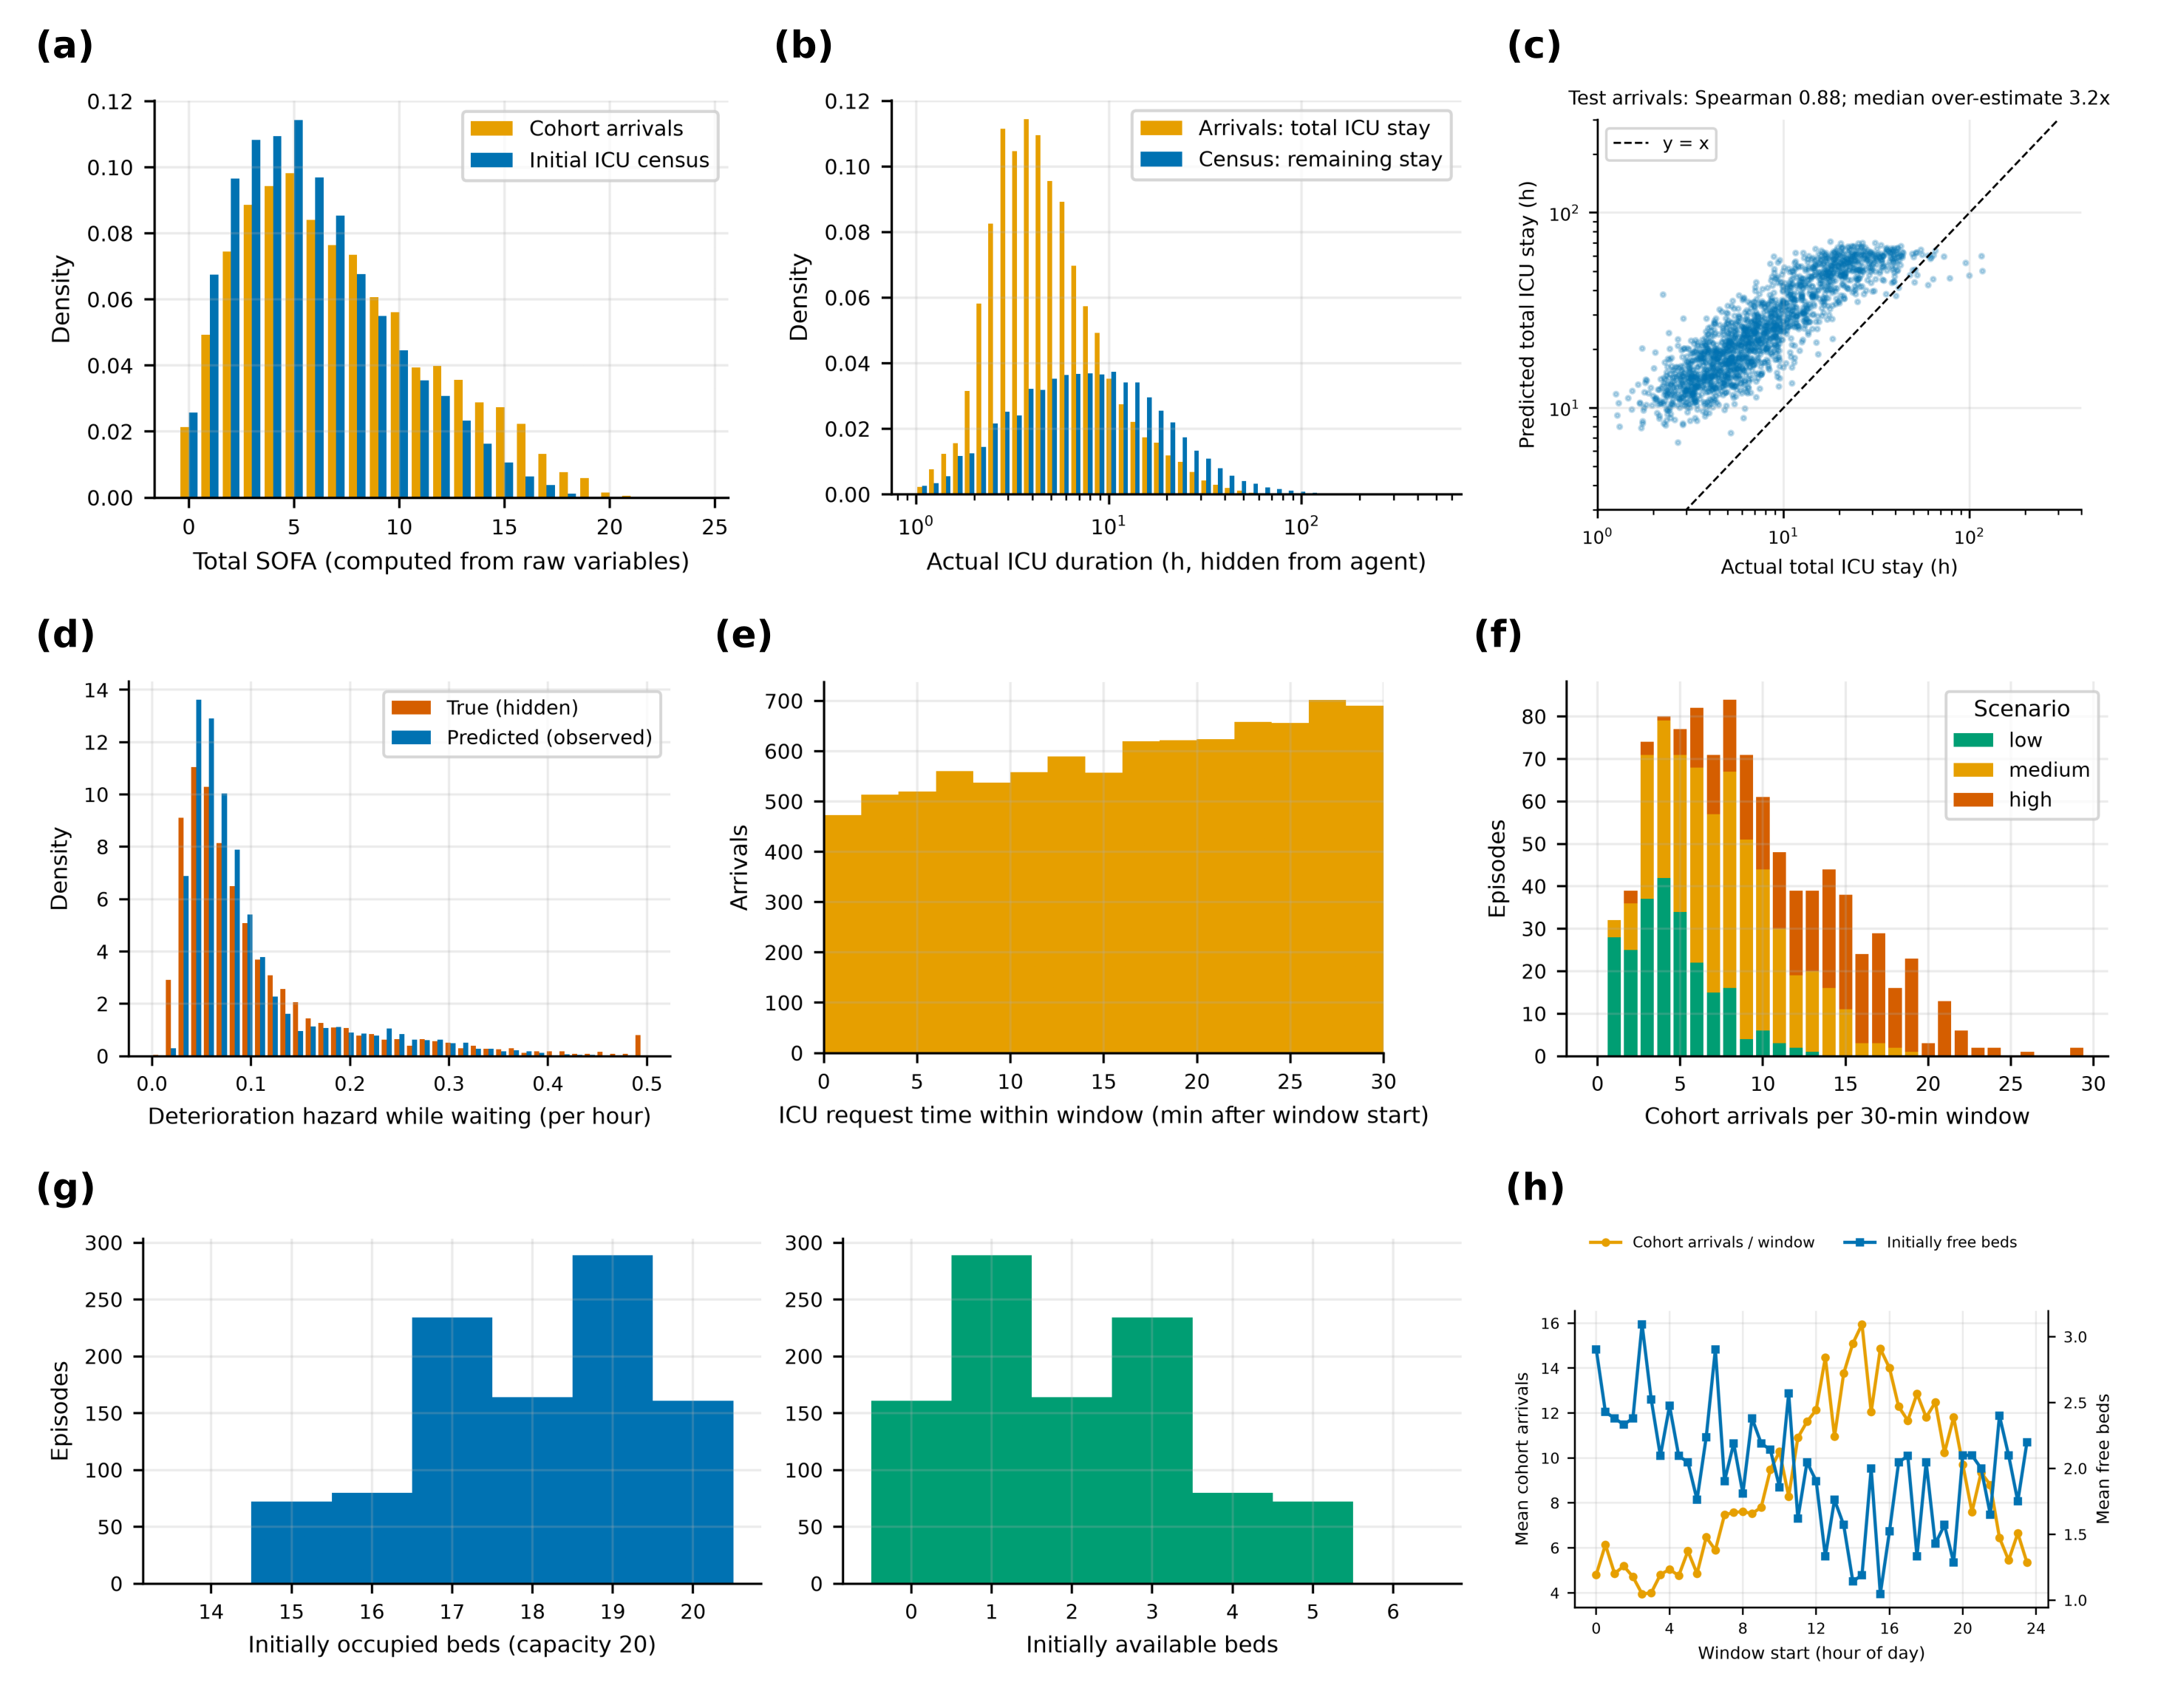
\includegraphics[width=\textwidth]{dataset_overview.png}
  \caption{Synthetic dataset. (a) Total SOFA computed from raw variables; (b) actual ICU durations (hidden from the agent); (c) predicted vs.\ actual total stay of test arrivals; (d) true and predicted deterioration hazard; (e) request times inside the 30-minute window; (f) cohort size per episode by congestion scenario; (g) initial occupancy and available beds; (h) mean cohort size and free beds for each of the 48 daily windows.}
  \label{fig:data}
\end{figure*}

\textbf{Windows throughout the day.} Episode $e$ uses the window slot $e \bmod 48$, so all 48 half-hour windows of a day (00:00--00:30 through 23:30--24:00) are represented about 21 times each. Each window is an independent synthetic draw with its own census, and consecutive windows are not chained. Demand varies with the hour $h$ of the window midpoint through $d(h)=\cos(2\pi(h-15)/24)$, which peaks at 15:00 and is lowest at 03:00. The expected number of arrivals is multiplied by $1+0.4\,d(h)$. Scenario probabilities are reweighted towards high congestion by the factor $1+0.5\,d$ and towards low congestion by $1-0.5\,d$. The mean cohort size therefore ranges from 4.0 arrivals (02:30 window) to 16.0 (14:30 window), and fewer beds are free in the afternoon (Fig.~\ref{fig:data}(h)). These are synthetic assumptions, not hospital statistics.

\textbf{Episodes and splits.} We generate 1{,}000 independent episodes: 700 for training, 100 for validation and 200 for testing, assigned at random by episode. Each has a 30-minute window, capacity $C=20$, and one of three congestion scenarios (low 235, medium 446, high 319 episodes). The scenario sets the number of initially free beds (low 3--5, medium 1--3, high 0--1) and the base mean cohort size (5, 8 and 12 arrivals). Overall there are on average 18.0 initially occupied beds (2.0 free) and 8.9 cohort arrivals (Fig.~\ref{fig:data}(f, g)).


\textbf{Existing ICU census.} For each episode we generate 18.0 occupants on average at the window start, each with a snapshot of raw measurements, an elapsed ICU time before the window start and a hidden remaining stay. Occupants are drawn with a length-biased stay (a census over-represents long stays), they are not counted as new arrivals, and they release beds when their hidden discharge time occurs.

\textbf{Cohort arrivals.} The number of arrivals is Poisson with a scenario-dependent mean (minimum one). Arrival times inside the window follow a non-homogeneous Poisson process with intensity proportional to $1+0.4\,t/T$ (rejection sampling, $T=30$ min), so arrivals are irregular and slightly more frequent late in the window (Fig.~\ref{fig:data}(e)).

\textbf{Raw clinical measurements.} A latent severity $z\in[0,1]$ (Beta(2,3); occupants scaled by 0.85) and patient-specific noise generate every raw variable via a deterministic function: PaO$_2$, FiO$_2$, PaO$_2$/FiO$_2$, ventilation, platelets, bilirubin, mean arterial pressure (MAP), vasopressor type and dose, Glasgow Coma Scale (GCS), creatinine, urine output, and also heart rate, respiratory rate, SpO$_2$, systolic/diastolic pressure and temperature (Fig.~\ref{fig:raw}). Age is drawn from a normal distribution (mean 62, SD 15, clipped to 18--95). Because the noise vector is fixed per patient, a later deterioration ($z\to z+\Delta z$) updates \emph{all} measurements coherently.

\textbf{SOFA from raw values.} The aggregate SOFA is never sampled. A separate module (\texttt{sofa\_calculator.py}) maps raw variables to six component scores (respiratory, coagulation, liver, cardiovascular, CNS, renal), each in $0$--$4$, and sums them:
\begin{equation}
  \mathrm{SOFA}_i=\sum_{j=1}^{6}\mathrm{SOFA}_{ij}\in\{0,\dots,24\}.
  \label{eq:sofa}
\end{equation}
In total there are 26{,}882 synthetic patients (8{,}881 arrivals, 18{,}001 census occupants). The mean SOFA of arrivals is 7.1, and 22.3\,\% of arrivals have SOFA $\ge 11$ (Fig.~\ref{fig:data}(a); components in Fig.~\ref{fig:comp}, Appendix). The raw measurements and all component scores are stored, and a validation test recomputes SOFA from the raw values and checks equality.

\textbf{Actual versus predicted ICU duration.} The actual total stay is lognormal,
$\log L_i=\log(8\,\mathrm{h})+3.0\,(z_i-0.4)+0.008\,(\mathrm{age}_i-62)+0.35\,(\mathrm{vent}_i-0.3)+0.3\,\varepsilon_i$ with $\varepsilon_i\sim\mathcal N(0,1)$; occupants' totals are multiplied by 3.0 (length bias) and their elapsed fraction is uniform on $[0.1,0.9]$ (Fig.~\ref{fig:data}(b)). The stay depends on severity but not through SOFA alone: other measurements and noise create variation among patients with equal SOFA. The agent never sees $L_i$. It sees a prediction from gradient-boosted regression trees~\cite{friedman2001gbm} (scikit-learn~\cite{pedregosa2011sklearn}) trained on raw measurements, SOFA components and age (plus elapsed time for occupants' remaining stay). Models are fitted \emph{on training episodes only}; training rows receive 5-fold out-of-fold predictions grouped by episode, and validation/test rows use the model fitted on all training rows. For test arrivals the predictions rank stays well (Spearman 0.88; 0.81 within an episode), but they are \emph{biased}: the total-stay model was fitted on arrivals and length-biased census patients together, so it overstates arrivals' stays by a median factor of 3.2 ($r^2=-1.35$ on $\log$-stay; Fig.~\ref{fig:data}(c)). The census remaining-stay model is calibrated ($r^2=0.54$). We found this error after all experiments and kept it, so the agent saw rank-preserving but inflated durations for waiting patients. The comparison between policies is unaffected because all of them saw the same features, but the absolute values of this feature are not comparable between waiting and ICU rows.

\textbf{Deterioration.} A hidden hazard $\lambda_i=\exp\{\log 0.03+2.2z_i+0.015(\mathrm{age}_i-62)+0.5\,\mathbb 1[\mathrm{SpO}_2<92]+f_i\}$ per hour, with patient frailty $f_i\sim\mathcal N(0,0.35^2)$, drives deterioration of waiting patients, with
\begin{equation}
  P(D_i\ \text{in}\ \Delta t)=1-e^{-\lambda_i\Delta t}.
  \label{eq:hazard}
\end{equation}
The agent sees only a \emph{predicted} hazard (test arrivals: $r^2=0.74$ on $\log\lambda$; Fig.~\ref{fig:data}(d)). A deterioration shifts $z$ by a random amount in $[0.08,0.18]$, so raw variables, SOFA, expected duration and predicted hazard are all recomputed. Deterioration times are generated from pre-drawn unit-exponential budgets, giving common random numbers across policies.

\textbf{Observable versus hidden data.} Observable files hold snapshots, census elapsed times, arrival timestamps (revealed only on arrival) and predictions. Hidden files hold actual stays, latent severity, noise, true hazards and deterioration budgets, and are read only by the simulator. A leakage audit (\texttt{dataset\_validation.py}) checks that observable files contain none of these columns, that predictions never equal actual values, that splits are disjoint by episode that all 48 windows are present and exactly 30 minutes long, and that seeds reproduce data (21 of 21 checks pass).

\textbf{Limitations of the dataset.} All distributions are assumptions; correlations are simpler than in real ICUs; stay lengths ignore mortality and transfers; and the congestion levels were adjusted by us to make the allocation problem learnable (see Section~\ref{sec:results}).

\begin{figure*}[!t]
  \centering
  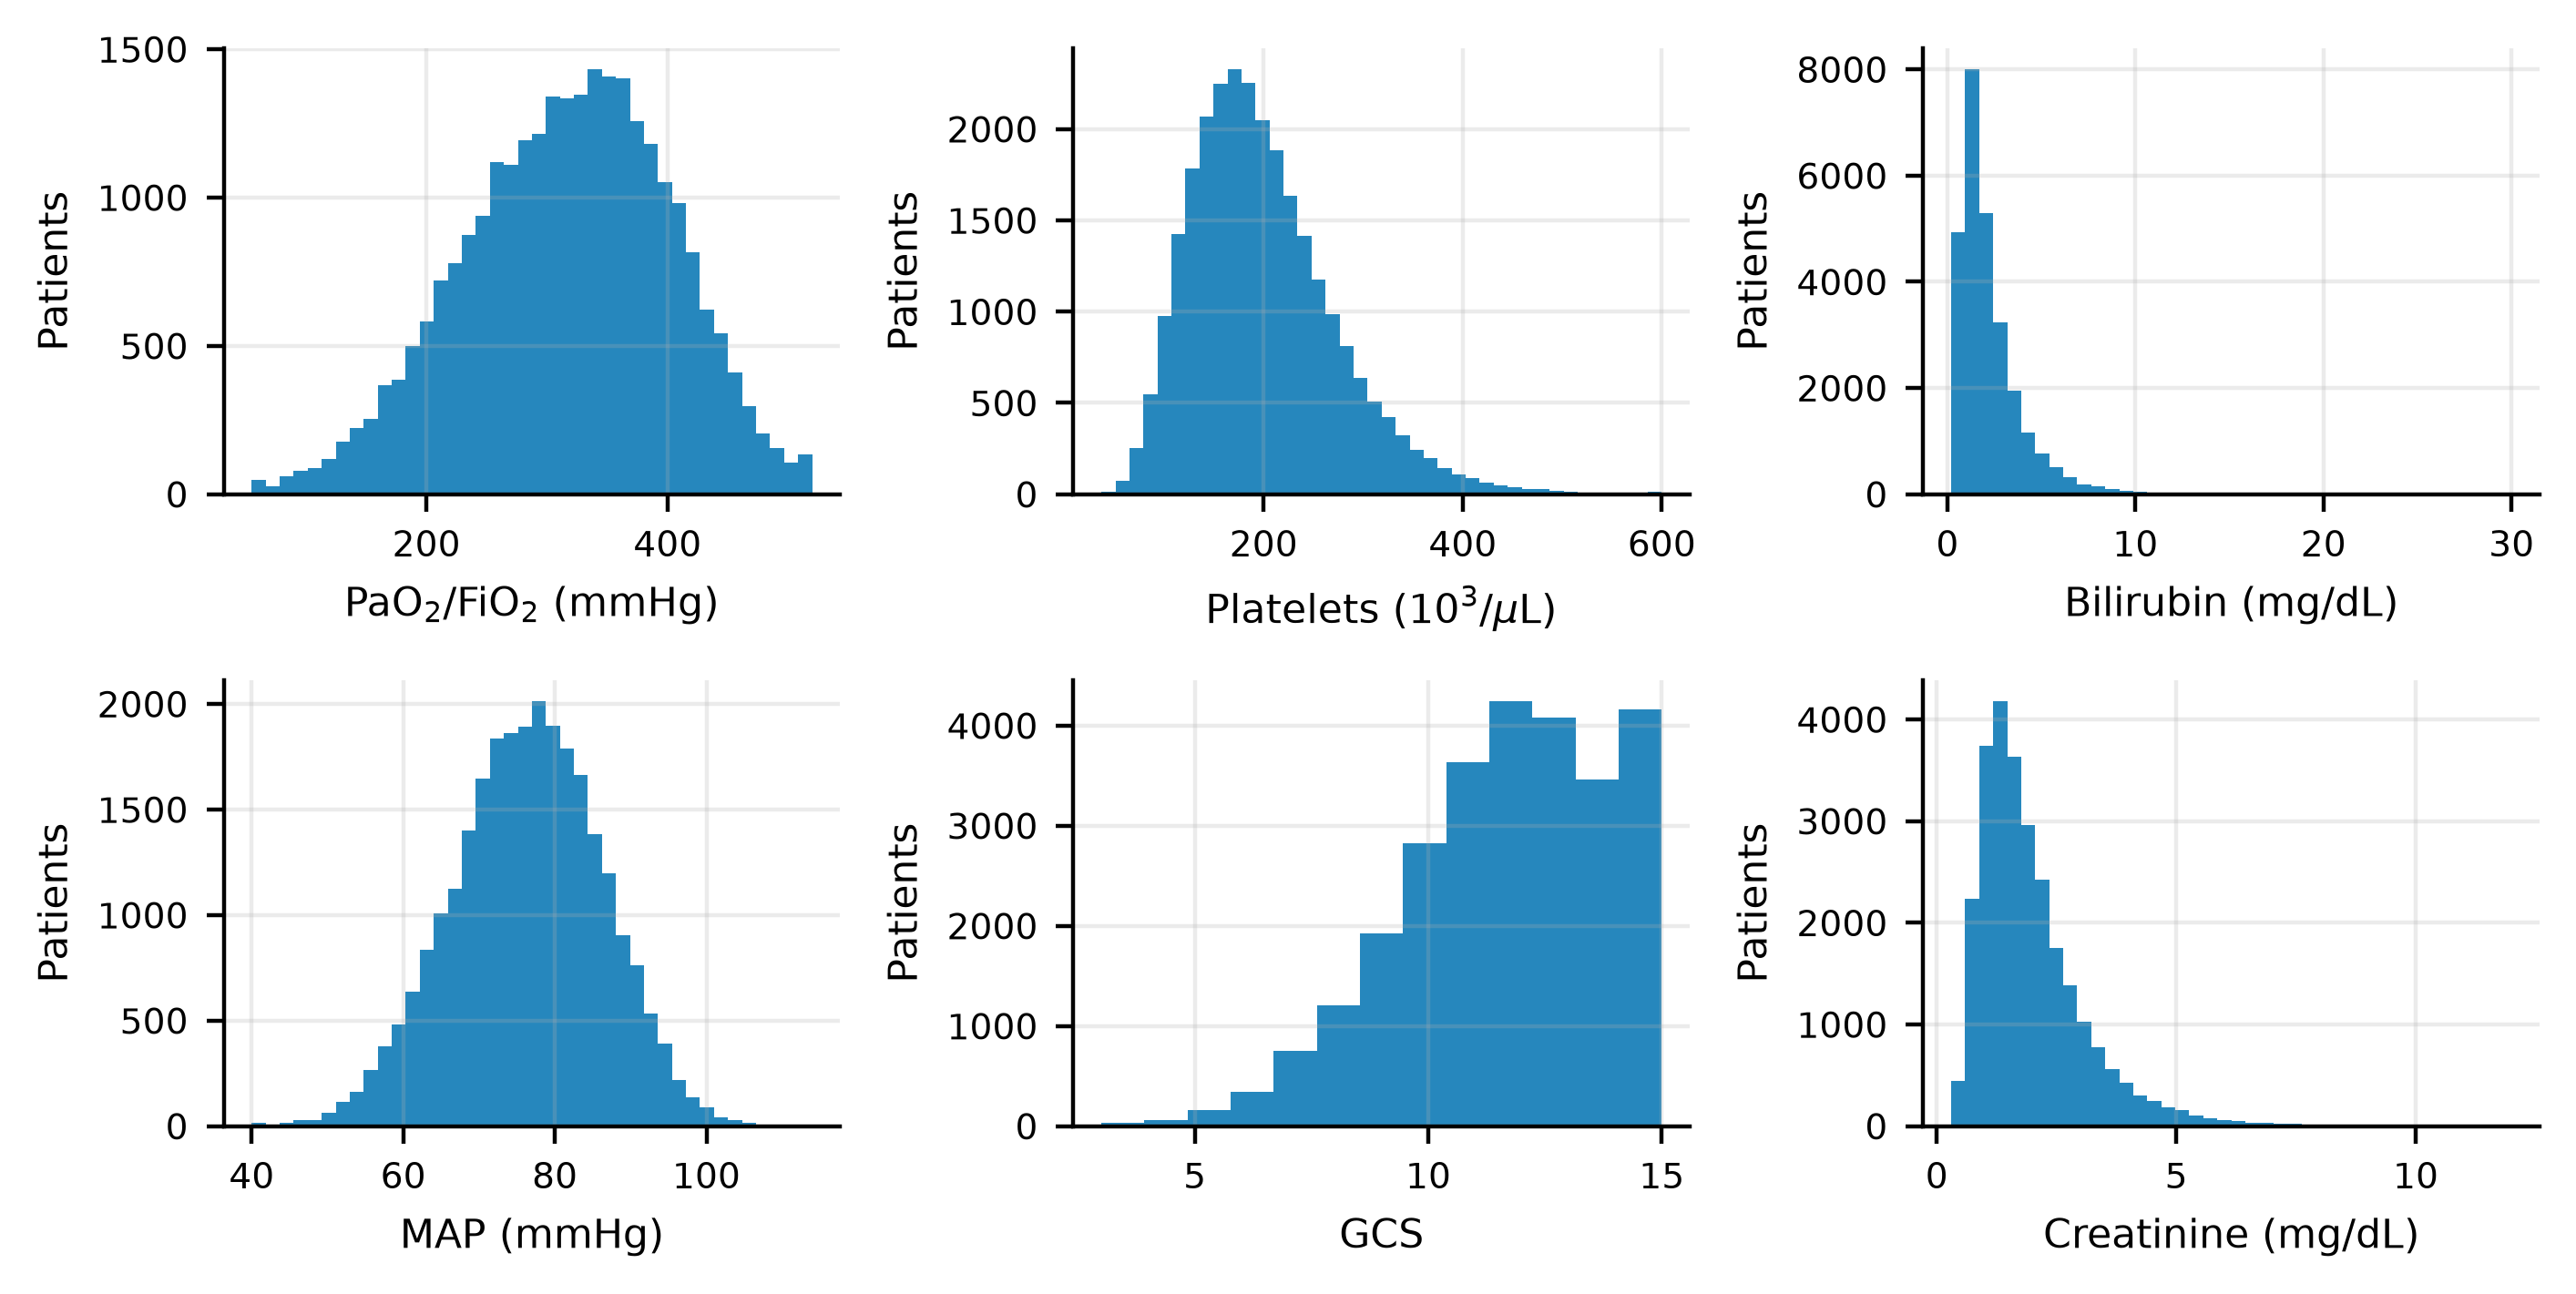
\includegraphics[width=0.72\textwidth]{raw_clinical_distributions.png}
  \caption{Distributions of six generated raw clinical variables (all synthetic patients).}
  \label{fig:raw}
\end{figure*}

\subsection{Problem Formulation: Markov Decision Processes}
\label{sec:mdp}
We model bed allocation as a semi-Markov decision process $\mathcal M=(\mathcal S,\mathcal A,P,R,\gamma)$, as shown in Fig.~\ref{fig:mdp}. The agent maximizes the expected discounted return
\begin{equation}
  G_t = \sum_{k=0}^{\infty} \gamma^{k} R_{t+k+1}, \qquad 0 \le \gamma < 1.
  \label{eq:return}
\end{equation}
The process is event-driven: the time between two decisions, $\Delta t=t_{next}-t$ in hours, is determined by the generated timestamps of arrivals, discharges and deteriorations, so $\Delta t$ varies. We therefore use the semi-Markov discount $\gamma^{\Delta t/\tau_0}$ with $\gamma=0.99$ and $\tau_0=1$ h~\cite{bradtke1995smdp}. Within a single decision epoch, when several patients are admitted one after another, $\Delta t=0$ and no discounting occurs. The 30-minute window is not a decision step: it only defines the cohort, and the episode continues after the window closes (Fig.~\ref{fig:window}). Time is measured in hours from the window start $T_e$.

\begin{figure*}[!t]
  \centering
  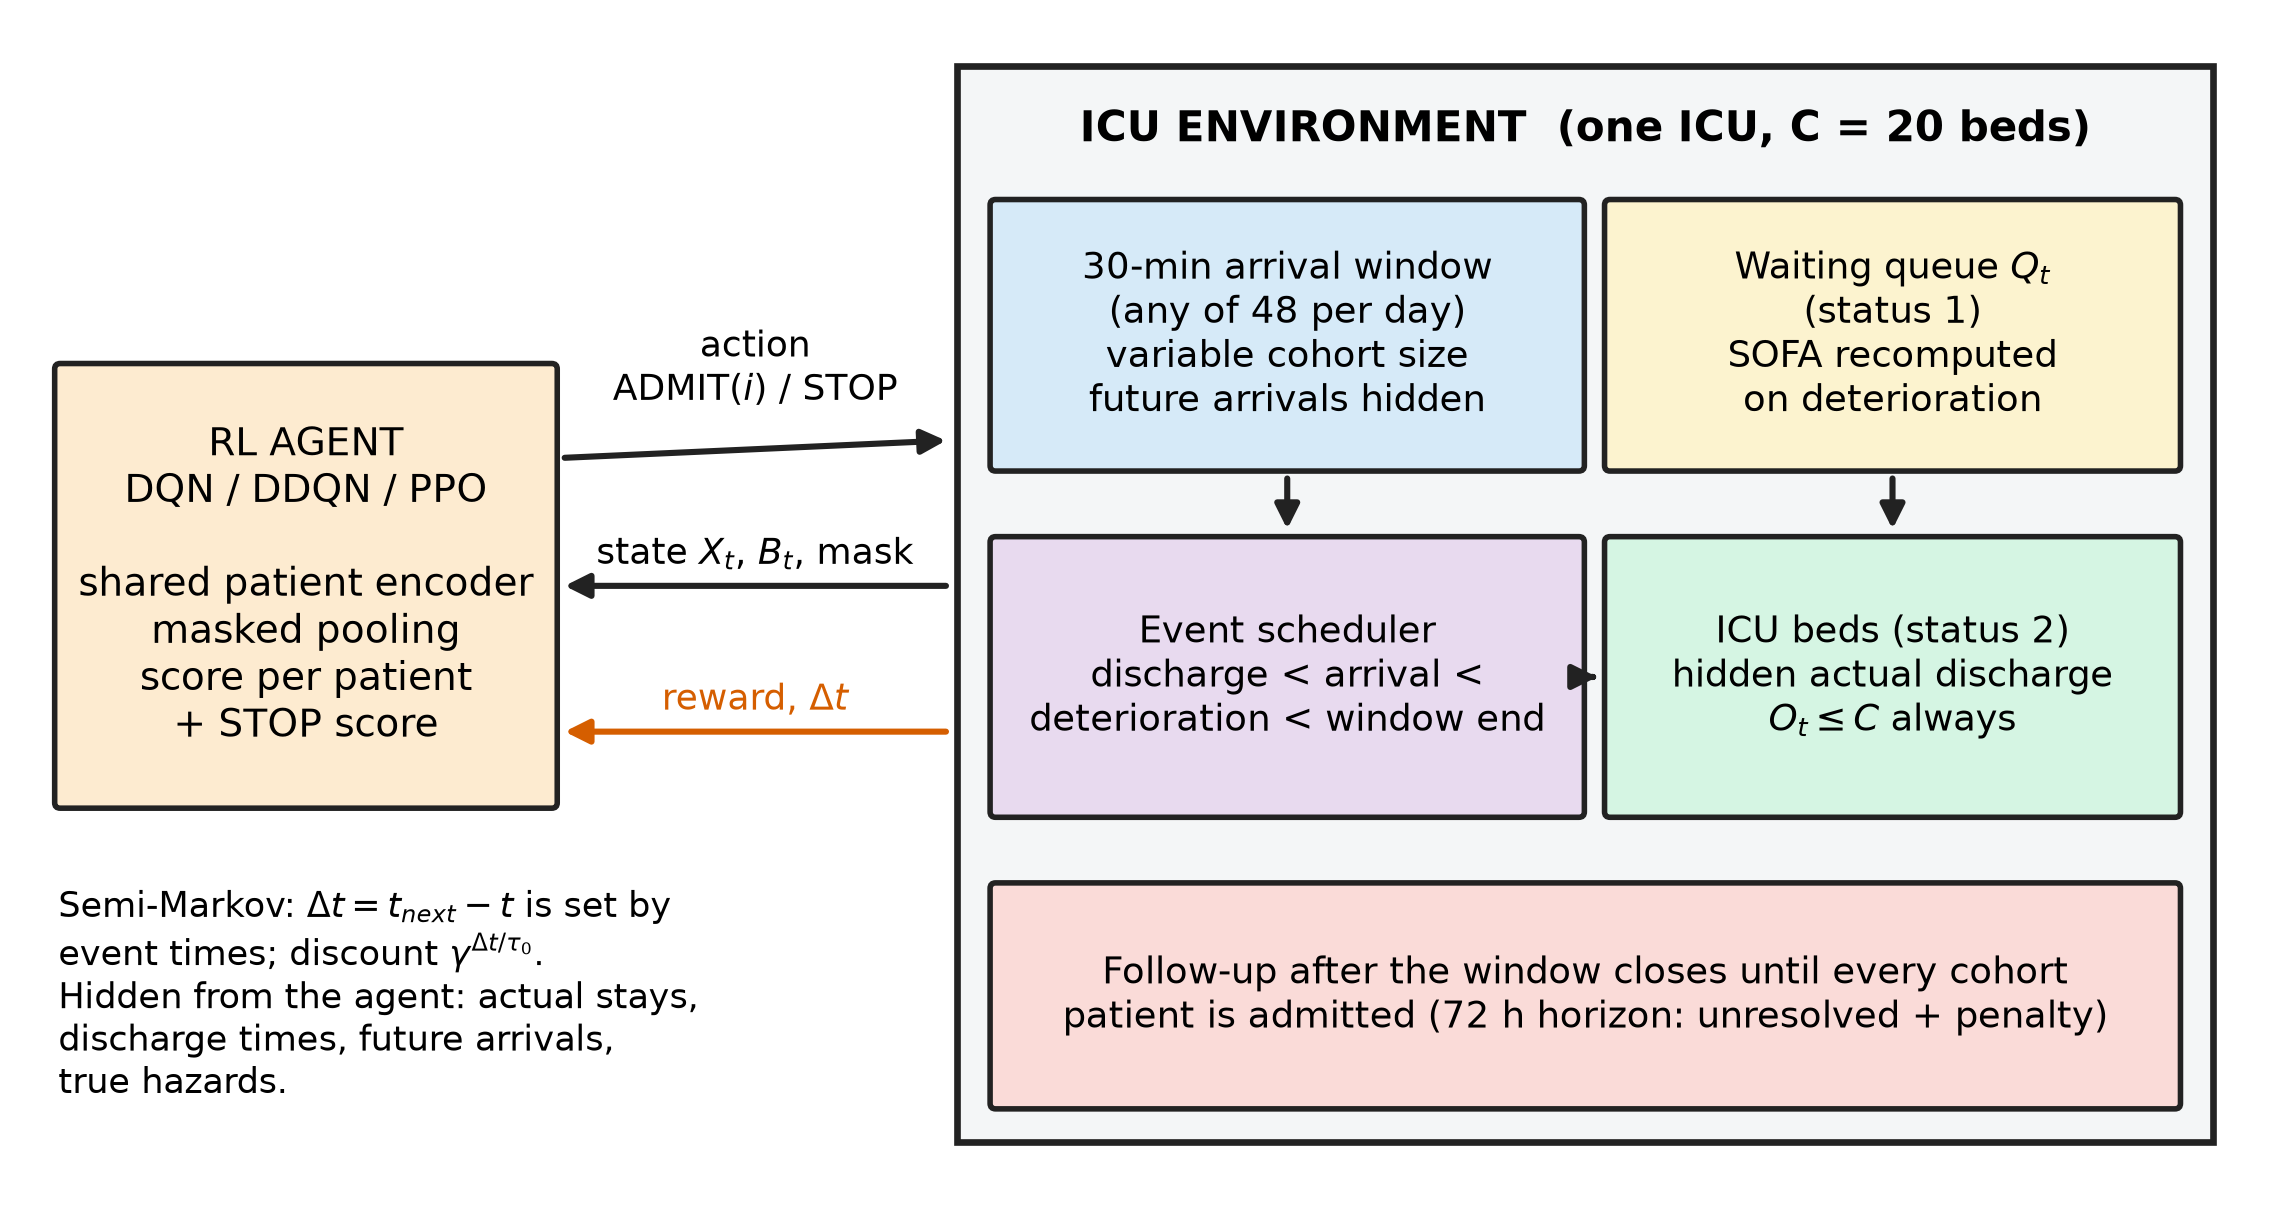
\includegraphics[width=0.85\textwidth]{mdp_diagram.png}
  \caption{Agent--environment interaction for the ICU problem. The agent observes the active patient matrix and free beds, and returns a masked admit/STOP action; the environment advances event by event and returns a reward integrated over the elapsed time.}
  \label{fig:mdp}
\end{figure*}
\begin{figure*}[!t]
  \centering
  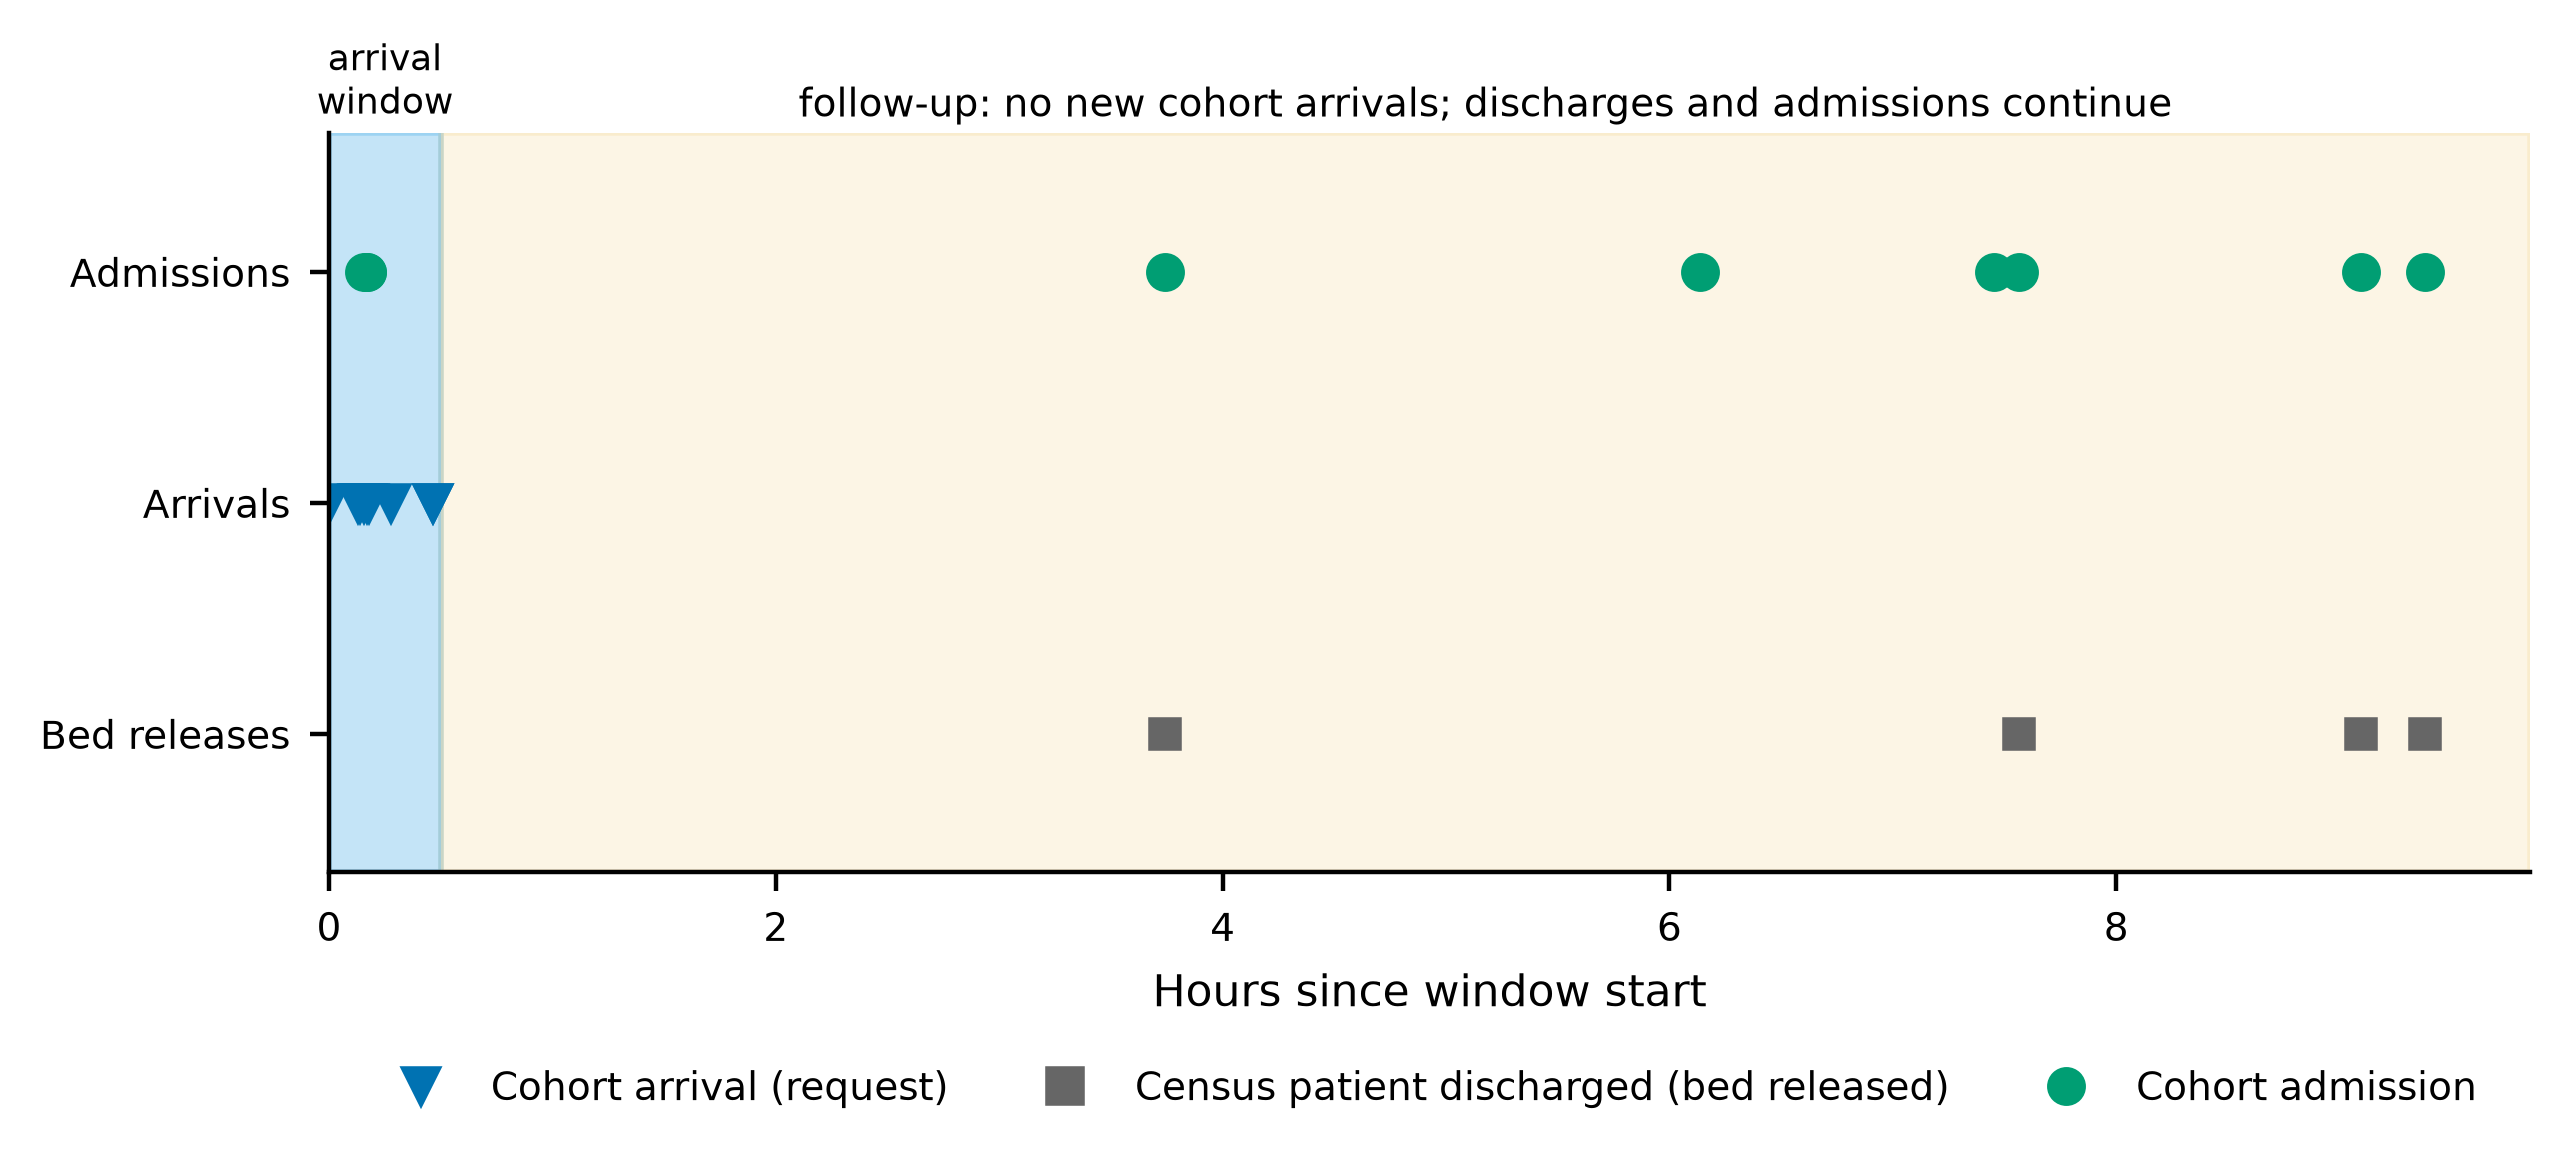
\includegraphics[width=0.85\textwidth]{arrival_window_diagram.png}
  \caption{Example test episode (10:30--11:00 window, DDQN): arrivals during the 30-minute window (shaded blue), then follow-up in which bed releases and admissions continue after the window has closed.}
  \label{fig:window}
\end{figure*}

\subsubsection{States}
At decision time $t$ the observation is a variable-size matrix
\begin{equation}
  X_t\in\mathbb R^{N_t\times 5},\qquad N_t=N_t^{ICU}+N_t^{Q},
  \label{eq:state}
\end{equation}
with one row per patient currently in an ICU bed ($N^{ICU}_t$) or arrived and waiting ($N^Q_t$). Each row holds five features: (1) SOFA, normalised $\mathrm{SOFA}/24$; (2) expected ICU bed-occupancy duration (predicted total stay if waiting, predicted remaining stay if in ICU), normalised by 48 h and clipped at 5; (3) waiting time $W_i(t)=t-t_i^{request}$ (zero for occupants), normalised by $W_{ref}=8$ h and clipped at 3; (4) predicted deterioration hazard (zero for occupants), normalised by 0.3~h$^{-1}$; (5) status, 1 = waiting and 2 = ICU, which is used as a categorical embedding and not as a number. The free bed count $B_t=C-N^{ICU}_t$ is passed as a global scalar $B_t/C$. Patients who have not arrived (status 0) and discharged patients (status 3) are absent, so $N_t$ grows with arrivals and shrinks with discharges. Patient identifiers are used only to map actions back to patients (Fig.~\ref{fig:state}). The simulator keeps four internal statuses: not arrived, waiting, in ICU, discharged.

The choice of five features keeps the state small: SOFA conveys severity, the predicted duration conveys how long a bed will be blocked, waiting time conveys fairness and urgency, hazard conveys expected deterioration, and status separates occupants from waiting candidates.

\begin{figure}[!t]
  \centering
  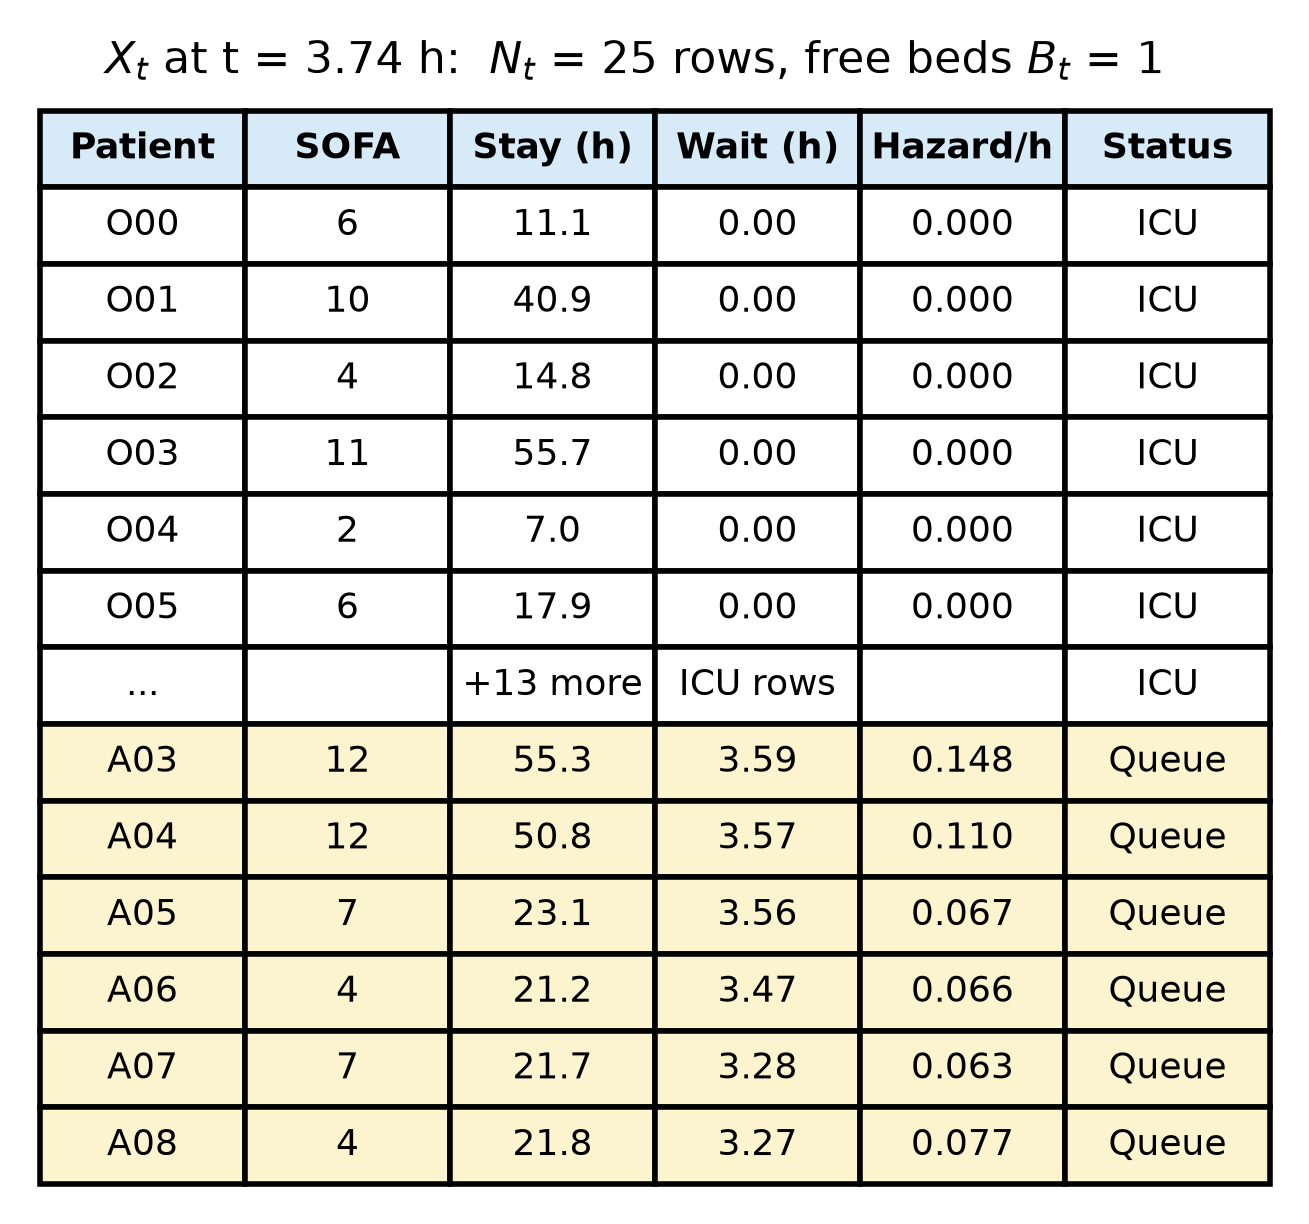
\includegraphics[width=0.95\columnwidth]{state_example.png}
  \caption{Example state matrix $X_t$ taken from a simulated episode: ICU occupants and queued candidates, with the quantities the agent actually observes.}
  \label{fig:state}
\end{figure}

\subsubsection{Actions}
Conceptually, each waiting patient receives an admit/wait decision $a_i\in\{0,1\}$, with the capacity constraint
\begin{equation}
  \sum_i a_{i,t}\le B_t.
  \label{eq:cap}
\end{equation}
Enumerating all $2^{N^Q_t}$ joint vectors is infeasible, so we use sequential masked selection. At a decision epoch (at least one free bed and at least one waiting patient) the agent chooses one action from
\begin{equation}
  \mathcal A_t=\{\mathrm{ADMIT}(i):i\in Q_t\}\cup\{\mathrm{STOP}\},
  \label{eq:actionset}
\end{equation}
and may choose again until the beds are full, the queue is empty or it selects STOP. Unselected patients remain waiting, so the sequence is equivalent to a binary vector satisfying \eqref{eq:cap}. The mask removes occupants, discharged and not-yet-arrived patients, and all patients when no bed is free. There is no pre-emption.

\subsubsection{Transition dynamics}
Events are processed in chronological order, and simultaneous events in a fixed order: ICU discharges (bed release), then cohort arrivals, then deteriorations, then window end. After a discharge the bed is available; an arrival sets the status to waiting and starts the waiting clock; a deterioration of a waiting patient updates raw variables, SOFA and the predictions. An admitted patient's hidden discharge is scheduled after its \emph{actual} stay, never its predicted stay. Formally, $(S_{t+1},\Delta t)\sim P(\cdot\mid S_t,A_t)$ (Fig.~\ref{fig:window}). The agent cannot see future arrivals, actual stays or true hazards. The simulator never lets occupancy exceed capacity (0 violations in all experiments).


\subsubsection{Episode termination}
After the window closes, an episode ends normally when all cohort patients have been admitted; patients already in ICU need not be simulated to discharge. A configurable maximum horizon of 72 h guards against stuck episodes: unresolved patients keep status waiting, are listed separately, their censored waiting time is $t_{horizon}-t_i^{request}$, and the terminal penalty $\lambda_UU_t$ is applied. In all reported test episodes every cohort patient was admitted (completion 100\,\%).

\textbf{Machine and software.} All experiments ran on an Apple M2 (8 CPU cores, 8 GB RAM, no CUDA GPU; computations on CPU) under macOS 14.5, with Python 3.12.6, PyTorch~\cite{paszke2019pytorch} 2.15.0, NumPy 2.5.4, pandas 3.1.0, scikit-learn 1.9.1, SciPy 1.18.1 and Matplotlib 3.11.2.

\subsection{Formulate reward}
Let $Q_t$ be the waiting set, $\Delta t$ the elapsed hours, $W_i(t)$ the waiting time, $U_t$ the number of patients unresolved at the horizon and $\lambda_U$ the terminal penalty coefficient.

\textbf{Reward 1: total waiting.} The cost between two events is the number of waiting patients times the elapsed time, i.e.\ the area under the queue-length curve,
\begin{equation}
  R_1(t)=-|Q_t|\,\Delta t-\lambda_UU_t.
  \label{eq:r1}
\end{equation}
For example, five patients waiting two hours cost $5\times2=10$ patient-hours. Summed over an episode, $-\sum_tR_1$ equals the total cumulative waiting time (up to the terminal term), so the reward is exactly aligned with the primary metric. It ignores severity on purpose.

\textbf{Reward 2: severity-weighted waiting.} With $\widetilde S_i=\mathrm{SOFA}_i/24$ and $\widetilde W_i(t)=\min(W_i(t)/W_{ref},1)$,
\begin{equation}
  R_2(t)=-\sum_{i\in Q_t}\int_{0}^{\Delta t}\!\big(\alpha\widetilde S_i+\beta\widetilde W_i(t+s)\big)\,ds-\lambda_UU_t.
  \label{eq:r2}
\end{equation}
Between events the queue and SOFA are constant and the waiting time grows linearly, so the integral has a closed form: $\alpha\widetilde S_i\Delta t+\beta\int_0^{\Delta t}\min\{(w_i+s)/W_{ref},1\}ds$, where $\int_0^{\Delta t}\min\{(w+s)/W_{ref},1\}ds=\frac{w\,\tau+\tau^2/2}{W_{ref}}+(\Delta t-\tau)$ with $\tau=\min\{\Delta t,\max(W_{ref}-w,0)\}$. This is implemented exactly (\texttt{reward\_functions.py}) and tested, not approximated with a fixed-step penalty. The defaults are $\alpha=\beta=1$ and $\lambda_U=30$ for both rewards, and rewards are multiplied by a scale (0.05 for $R_1$, 0.1 for $R_2$) only for numerical conditioning. Rewards are finite, capacity is a hard constraint of the simulator, and nothing rewards filling beds. $R_1$ suits a hospital manager who wants to minimise aggregate delay; $R_2$ suits a clinician who also wants severe patients not to wait. The two are different objectives and neither is assumed to be better.

\subsection{Establish value functions (in terms of your environmental variables)}
For a state $s$ (the matrix $X_t$ plus free beds) and a selection action $a$ (admit patient $i$ or STOP), the action-value function satisfies the Bellman optimality equation
\begin{equation}
  Q^{*}(s,a) = \mathbb{E}\!\left[ R_{t+1} + \gamma \max_{a'} Q^{*}(S_{t+1}, a') \,\middle|\, S_t = s, A_t = a \right].
  \label{eq:bellman}
\end{equation}
Equation~\eqref{eq:bellman} follows from \eqref{eq:return}; see Section~\ref{sec:mdp}. Because decisions are separated by random event durations, the discount depends on the elapsed time,
\begin{equation}
  Q^*(s,a)=\mathbb E\!\left[r+\gamma^{\Delta t/\tau_0}\max_{a'}Q^*(s',a')\right],
  \label{eq:smdpq}
\end{equation}
where $r$ is the reward accumulated over the elapsed time (waiting cost in patient-hours for $R_1$), $\Delta t$ is the time to the next decision epoch (zero when another patient is admitted at the same epoch), $s'$ is the next state and $a'$ ranges over the masked action set. The state value is $V(s)=\max_aQ^*(s,a)$.

\subsection{RL Algorithms used in your project}
All learners share the \emph{same} environment, action interface and network body.

\textbf{Network.} The number of rows varies, so we use a permutation-equivariant set network in the spirit of Deep Sets~\cite{zaheer2017deepsets}. A shared MLP encodes each row (four normalised features plus an 8-dimensional status embedding, two layers of 64 units), masked mean and max pooling over active rows plus the free-bed fraction form a context vector (64 units), a head maps [row encoding, context] to a score for each row, and a separate head maps the context to a STOP score. The scores are $Q$-values for DQN/DDQN and logits for PPO; PPO's critic is a separate head on the context vector. Invalid actions receive $-10^{9}$ before the arg-max/softmax. Patient order and identifiers cannot influence the output, and padding rows are masked.

\textbf{Random baseline.} Chooses uniformly among eligible waiting patients (never STOP) until the beds are full or the queue is empty, five seeds. We also report two transparent non-learning heuristics for context: shortest predicted stay first (SPF) and highest SOFA first.

\textbf{DQN.} Q-network, target network (hard update every 250 updates), replay buffer (50{,}000), $\epsilon$-greedy exploration (1.0 to 0.05 over 40\,\% of training, with STOP chosen with probability 0.05 when exploring), Adam~\cite{kingma2015adam} (lr $10^{-3}$), batch 64, Huber loss, duration-aware target $y=r+\gamma^{\Delta t/\tau_0}\max_{a'}Q_{\bar\theta}(s',a')$ over valid $a'$ and no bootstrap at termination~\cite{mnih2015dqn}.

\textbf{DDQN.} The same except that the online network selects the next action and the target network evaluates it, $y=r+\gamma^{\Delta t/\tau_0}Q_{\bar\theta}(s',\arg\max_{a'}Q_\theta(s',a'))$, which reduces overestimation~\cite{vanhasselt2016ddqn}.

\textbf{PPO.} A masked categorical policy over $\{\mathrm{ADMIT}(i)\}\cup\{\mathrm{STOP}\}$, a critic, clipped surrogate $L=\mathbb E[\min(\rho_tA_t,\mathrm{clip}(\rho_t,1\pm0.2)A_t)]$ with $\rho_t=\pi_\theta/\pi_{old}$, value loss (0.5), entropy bonus (0.01), generalised advantage estimation~\cite{schulman2016gae} with a duration-aware discount $\gamma_t=\gamma^{\Delta t_t/\tau_0}$: $\delta_t=r_t+\gamma_tV(s_{t+1})-V(s_t)$, $A_t=\delta_t+\gamma_t\lambda A_{t+1}$ with $\lambda=0.95$ \cite{schulman2017ppo}. Updates occur every 32 episodes (4 epochs, minibatch 256, lr $3\times10^{-4}$).

\textbf{Why these algorithms.} DQN and DDQN are value-based with a discrete masked action set, which suits ``pick one patient''; PPO is a stable on-policy alternative with a learned critic that can absorb episode-level variance. Pseudocode is in the Appendix.

\section{Results}\label{sec:results}
\begin{table*}[!t]
  \caption{Held-out test results, Reward~1 (200 episodes over all daily windows; mean over 5 seeds, $\pm$ SD across seeds for total wait; heuristics are deterministic). Lower is better except return.}
  \label{tab:results}
  \centering
  \footnotesize
  \setlength{\tabcolsep}{4pt}
  \begin{tabular}{lcccccccc}
    \toprule
    \textbf{Policy} & \textbf{Total wait} & \textbf{Mean wait} & \textbf{Max wait} & \textbf{High-SOFA} & \textbf{Sev.-wtd} & \textbf{Det.} & \textbf{Util.} & \textbf{Return} \\
     & (patient-h) & (h) & (h) & \textbf{wait (h)} & \textbf{cost} & \textbf{events} & & \\
    \midrule
    Random      & 60.40 $\pm$ 0.30 & 4.903 & 8.732 & 5.417 & 72.23 & 6.41 & 0.982 & $-3.020$ \\
    DQN         & \textbf{57.34 $\pm$ 0.71} & 4.877 & \textbf{8.581} & 6.764 & \textbf{69.41} & 6.66 & 0.973 & $\mathbf{-2.867}$ \\
    DDQN        & 57.74 $\pm$ 0.63 & 4.872 & 8.614 & 6.425 & 69.84 & 6.60 & 0.974 & $-2.887$ \\
    PPO         & 59.37 $\pm$ 6.15 & \textbf{4.818} & 8.649 & 5.466 & 70.93 & 6.46 & 0.982 & $-2.969$ \\
    \midrule
    SPF heuristic & 54.98 & 4.532 & 8.116 & 6.425 & 66.79 & 6.69 & 0.982 & $-2.749$ \\
    SOFA-first heuristic & 67.87 & 5.386 & 9.724 & 2.984 & 78.24 & 6.34 & 0.982 & $-3.393$ \\
    \bottomrule
  \end{tabular}
\end{table*}

\begin{table}[!t]
  \caption{Selection criteria (5 seeds, mean $\pm$ SD).}
  \label{tab:select}
  \centering
  \footnotesize
  \setlength{\tabcolsep}{3pt}
  \begin{tabular}{lccc}
    \toprule
    \textbf{Criterion} & \textbf{DQN} & \textbf{DDQN} & \textbf{PPO} \\
    \midrule
    Conv.\ episode (seeds) & 1667 (3/5) & 500 (2/5) & 2133 (3/5) \\
    Train time (s) & 1338 $\pm$ 53 & 1371 $\pm$ 87 & 312 $\pm$ 56 \\
    Test total wait & 57.34 $\pm$ 0.71 & 57.74 $\pm$ 0.63 & 59.37 $\pm$ 6.15 \\
    Seeds better than Random & 5/5 & 5/5 & 3/5 \\
    Val.\ plateau return & $-3.69$ & $-3.70$ & $-3.66$ \\
    \bottomrule
  \end{tabular}
\end{table}

\textbf{Protocol.} All learners were trained with Reward~1 for the same budget of 6{,}000 training episodes, sampled from the 700 training episodes (all 48 daily windows), with five seeds each (0--4). They were validated every 200 episodes on the 100 validation episodes. For each run the checkpoint with the best validation return was kept (selection on validation only), and every policy was evaluated once on the same 200 held-out test episodes (mean 9.13 cohort patients, all times of day). High-SOFA patients are those with SOFA $\ge11$ at arrival. This threshold, motivated by the highest mortality band of~\cite{ferreira2001serial}, was fixed before training.

\textbf{Development history (disclosure).} The study went through four full runs. (i)~With only the 10:00--10:30 window and an easier scenario, a 2{,}500-episode run gave learned policies that did \emph{not} beat Random (test total wait: PPO 26.1, DDQN 27.0, DQN 28.2, Random 25.6 patient-hours). (ii)~After diagnosis we changed the setup, using validation episodes only. DQN/DDQN had selected STOP in 26--41\,\% of decisions, and the best ordering gain was only about 4\,\%, small against episode-to-episode variance. We made stays more severity-dependent and predictable, increased congestion, lowered STOP sampling during DQN exploration and raised the budget to 6{,}000 episodes. A run with final checkpoints was still worse than Random for all learners. (iii)~Best-validation checkpointing and larger, slower PPO updates gave PPO 53.3 vs.\ Random 57.2 on the 10:00 window. (iv)~The design was then extended to all 48 daily windows with time-of-day demand, and everything was retrained with unchanged hyperparameters. Only run (iv) is reported below. Earlier outputs are archived in \texttt{results/archive\_*}. The test set was never used to choose settings. However, the synthetic assumptions \emph{were} changed to make the problem learnable, and test results were inspected after each full run, so the effect sizes describe this tuned simulator only.

\subsection*{1) Convergence of the algorithms}
Fig.~\ref{fig:conv} shows the validation return (mean of five seeds, shaded $\pm1$ SD) against the Random reference ($-3.69$). Convergence is the first evaluation at which a run closes 95\,\% of the gap between Random and its own plateau (mean of its last five evaluations); runs whose plateau does not exceed Random never converge. The curves are noisy because validation episodes differ greatly in congestion. DDQN first reaches the reference level after about 2{,}000 episodes, DQN after about 2{,}600, and both then fluctuate around it. PPO's mean stays below the reference until about 5{,}000 episodes, with a wide band. By the criterion, DDQN converges after $500\pm707$ episodes (2 of 5 seeds), DQN after $1{,}667\pm1{,}447$ (3/5) and PPO after $2{,}133\pm2{,}656$ (3/5). Plateau returns are $-3.69\pm0.13$ (DDQN), $-3.69\pm0.12$ (DQN) and $-3.66\pm0.43$ (PPO). The validation curves use the network at each evaluation, while the test results use each run's best-validation checkpoint, so test performance is better than the late curves suggest.


\begin{figure*}[!t]
  \centering
  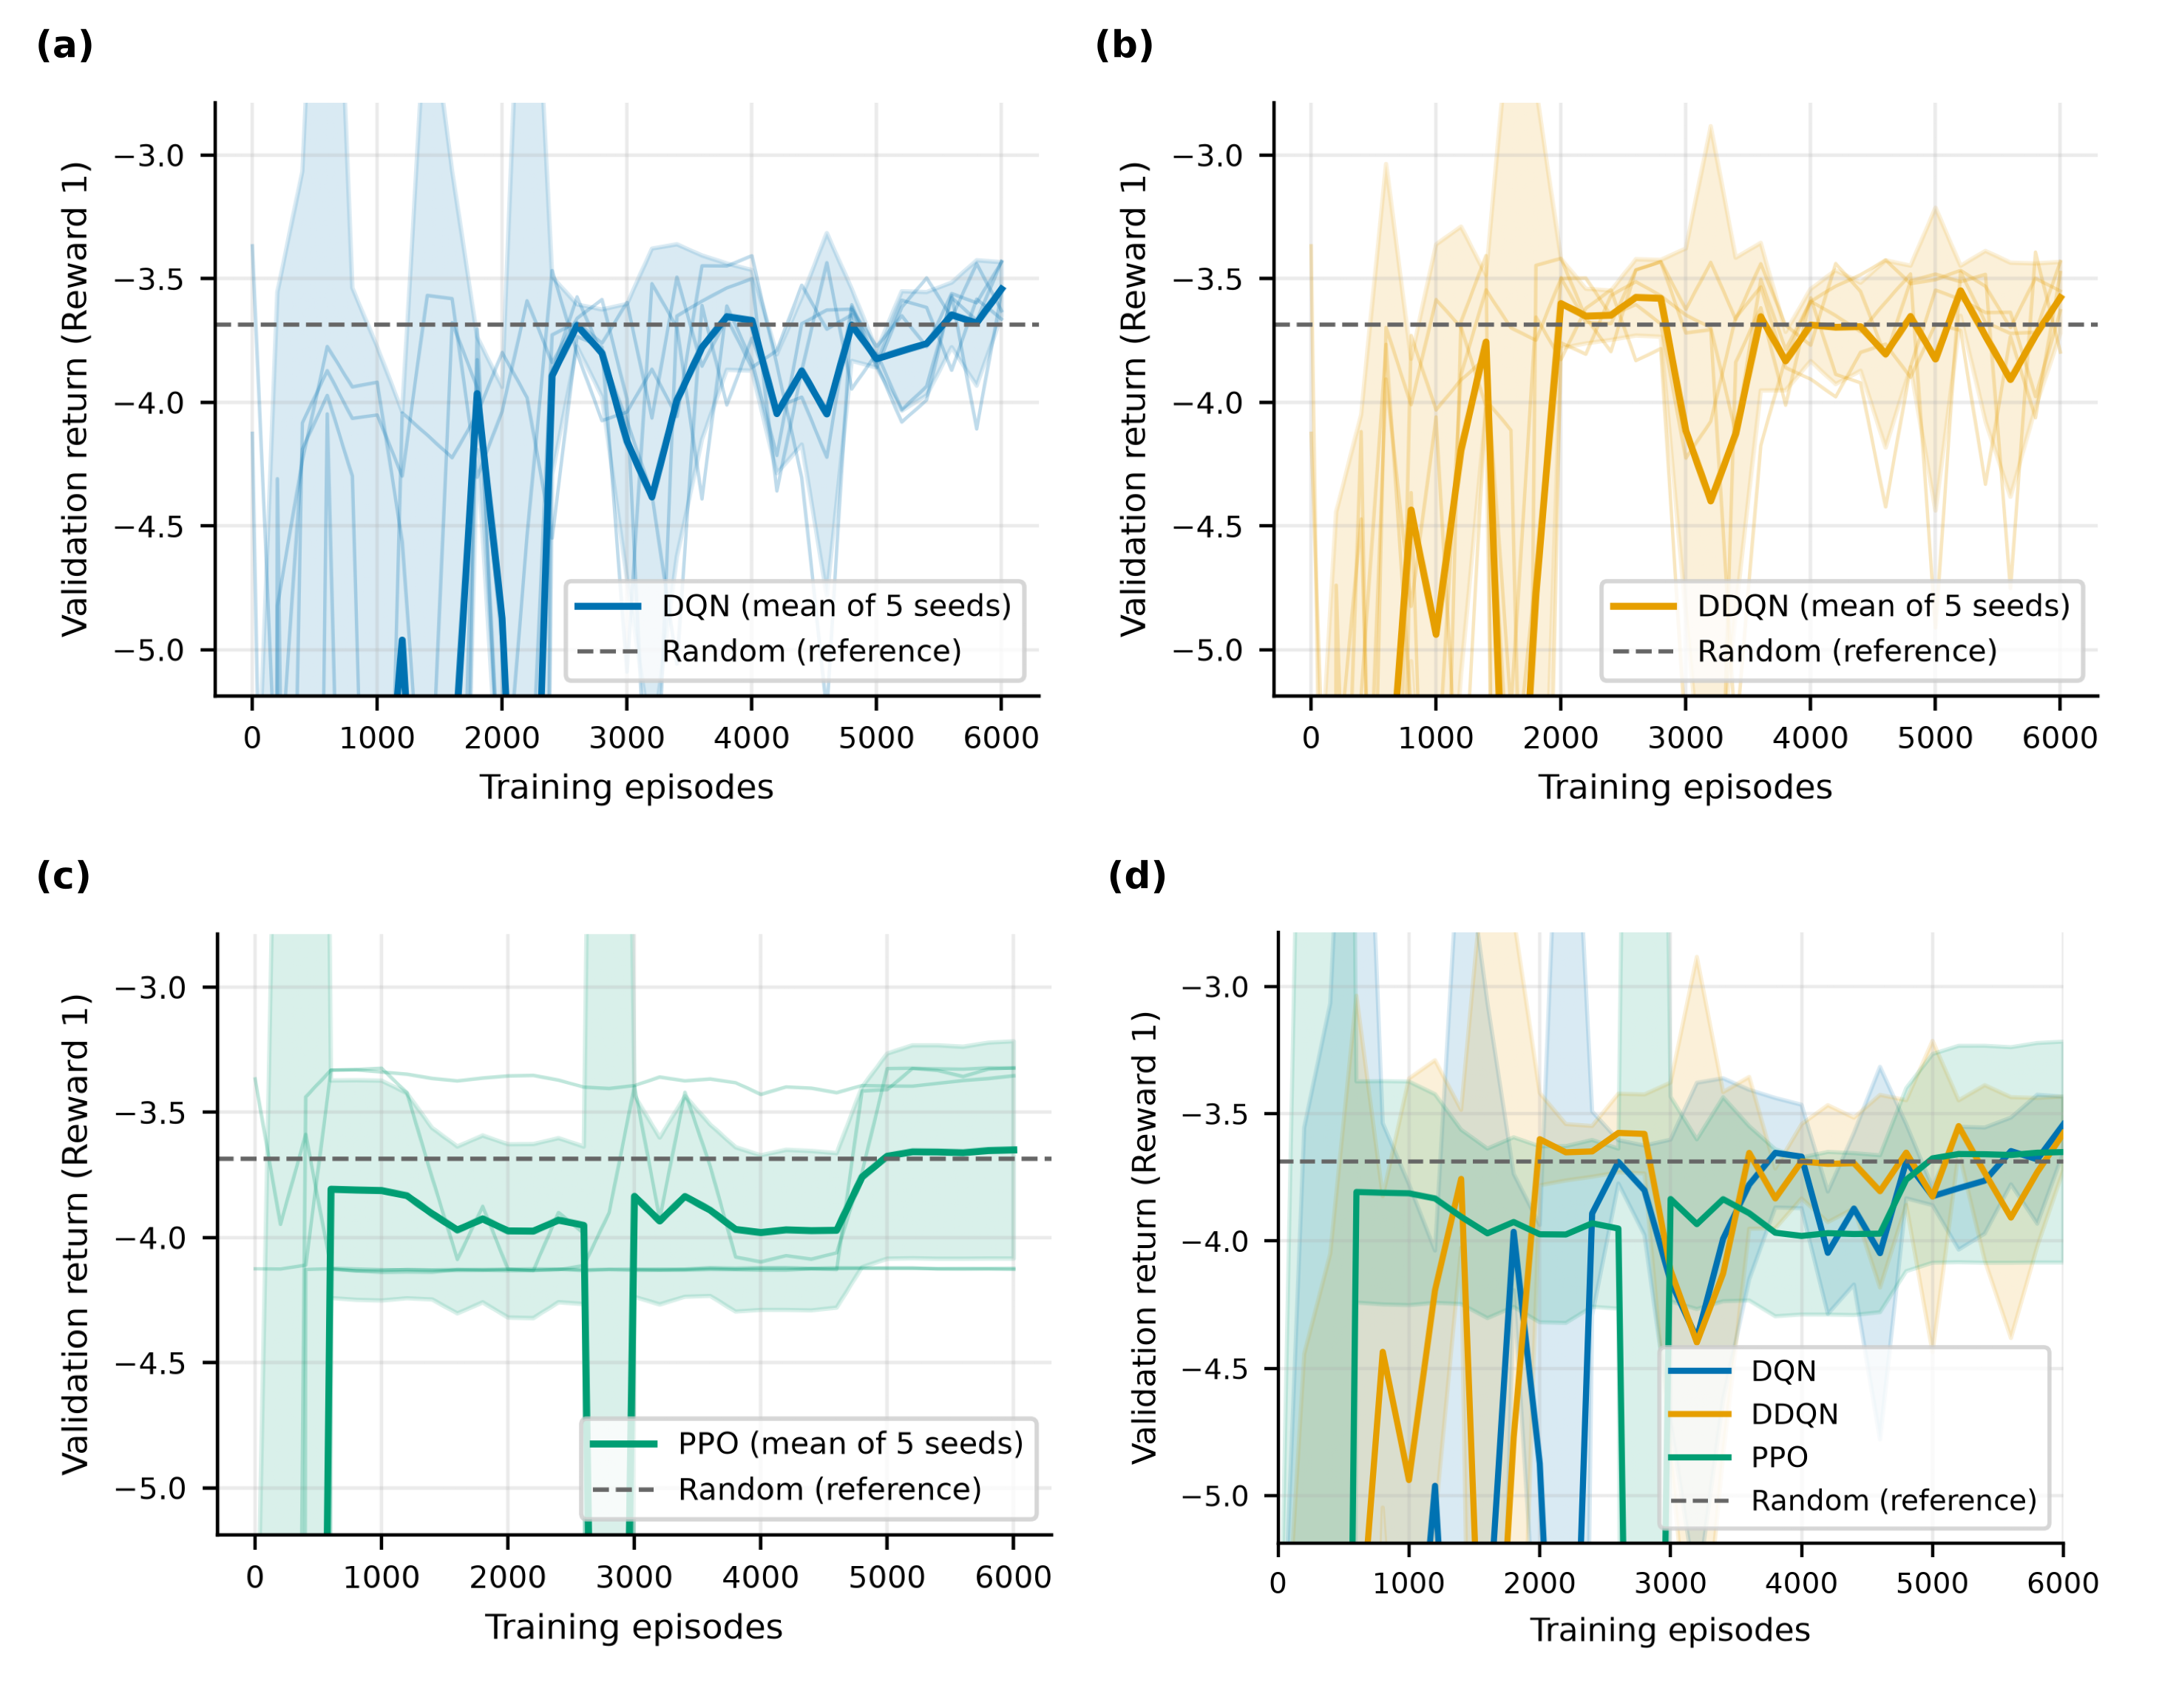
\includegraphics[width=0.86\textwidth]{convergence_all.png}
  \caption{Validation return during training (mean of five seeds, band $\pm1$ SD; thin lines: seeds) for (a) DQN, (b) DDQN, (c) PPO, and (d) all three; dashed line: Random reference.}
  \label{fig:conv}
\end{figure*}

Table~\ref{tab:results} gives the held-out results. Admission completion is 100\,\%, unresolved patients 0 and capacity violations 0 for every policy. We pair over the 200 test episodes and report bootstrap 95\,\% CIs of the per-episode difference to Random in total waiting. The changes are $-3.06$ [$-4.13,-2.00$] for DQN, $-2.67$ [$-3.57,-1.78$] for DDQN, $-1.03$ [$-1.42,-0.67$] for PPO and $-5.42$ [$-6.90,-4.12$] for the shortest-predicted-first (SPF) heuristic. All learners therefore improve on Random, by 5.1\,\% (DQN), 4.4\,\% (DDQN) and 1.7\,\% (PPO). None of them reaches the simple SPF rule (9.0\,\%), so we do not claim that RL is necessary for Reward~1. The mechanism is visible in the high-SOFA column. Gains in total waiting come from admitting short predicted stays first, which frees beds sooner, and they are paid for by longer waits of high-SOFA patients (DQN 6.76 h vs.\ Random 5.42 h). PPO behaves bimodally. Seeds 0, 1 and 3 reach 55.2, 55.0 and 55.0 patient-hours, matching the SPF heuristic and the best of all runs. Seeds 2 and 4 collapse to 68.2 and 63.6, worse than Random. All metrics are compared in Fig.~\ref{fig:cmp}.


\begin{figure*}[!t]
  \centering
  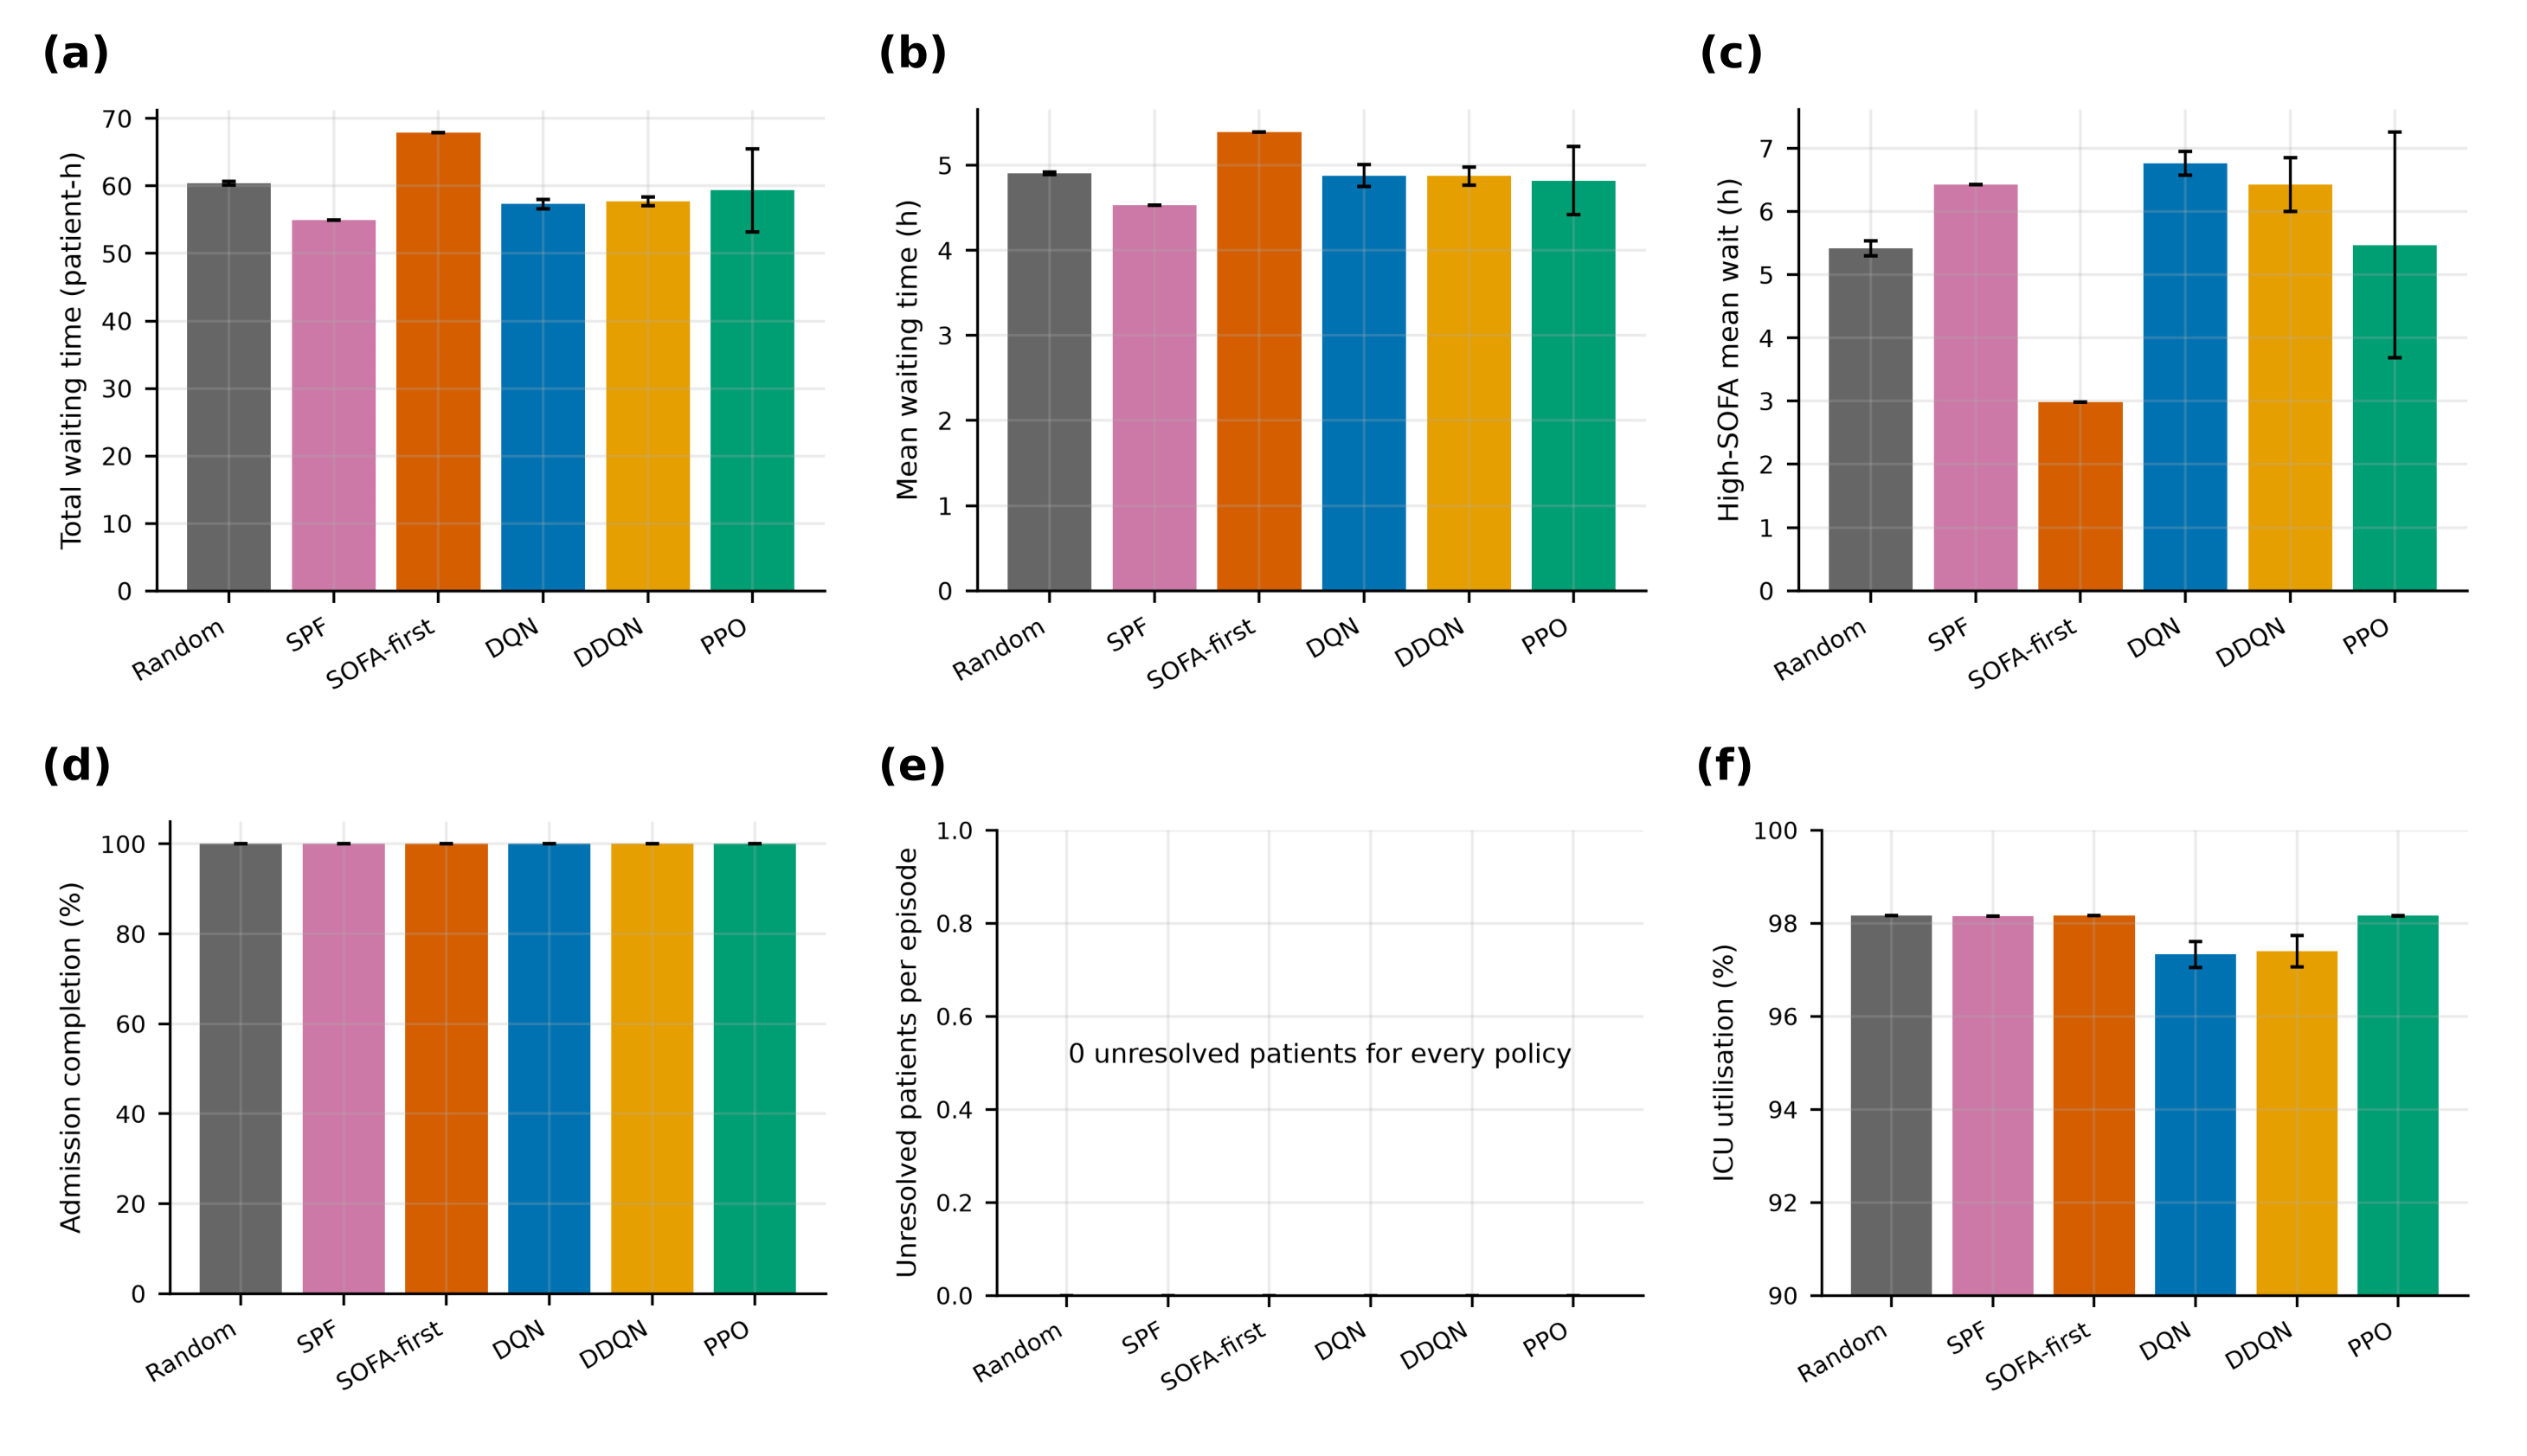
\includegraphics[width=0.92\textwidth]{algorithm_comparison.png}
  \caption{Test-set comparison (mean over seeds, error bars: SD across seeds): (a) total waiting, (b) mean waiting, (c) high-SOFA waiting, (d) admission completion, (e) unresolved patients, (f) time-weighted ICU utilisation (descriptive only).}
  \label{fig:cmp}
\end{figure*}

\textbf{Agent snapshots.} Fig.~\ref{fig:snap} shows test episode 21 (10:30--11:00 window, medium congestion, 9 cohort patients, 3 free beds). It was chosen by a fixed rule, the first medium-congestion test episode with 6--9 arrivals and at least 2 free beds, without looking at performance. DDQN admits the patients with short predicted stays early and leaves long-stay, high-SOFA patients (A01, A02) waiting longest. In this particular episode its total wait (41.9 patient-hours) is slightly \emph{worse} than Random's (41.5): the average advantage in Table~\ref{tab:results} does not hold in every episode.

\begin{figure*}[!t]
  \centering
  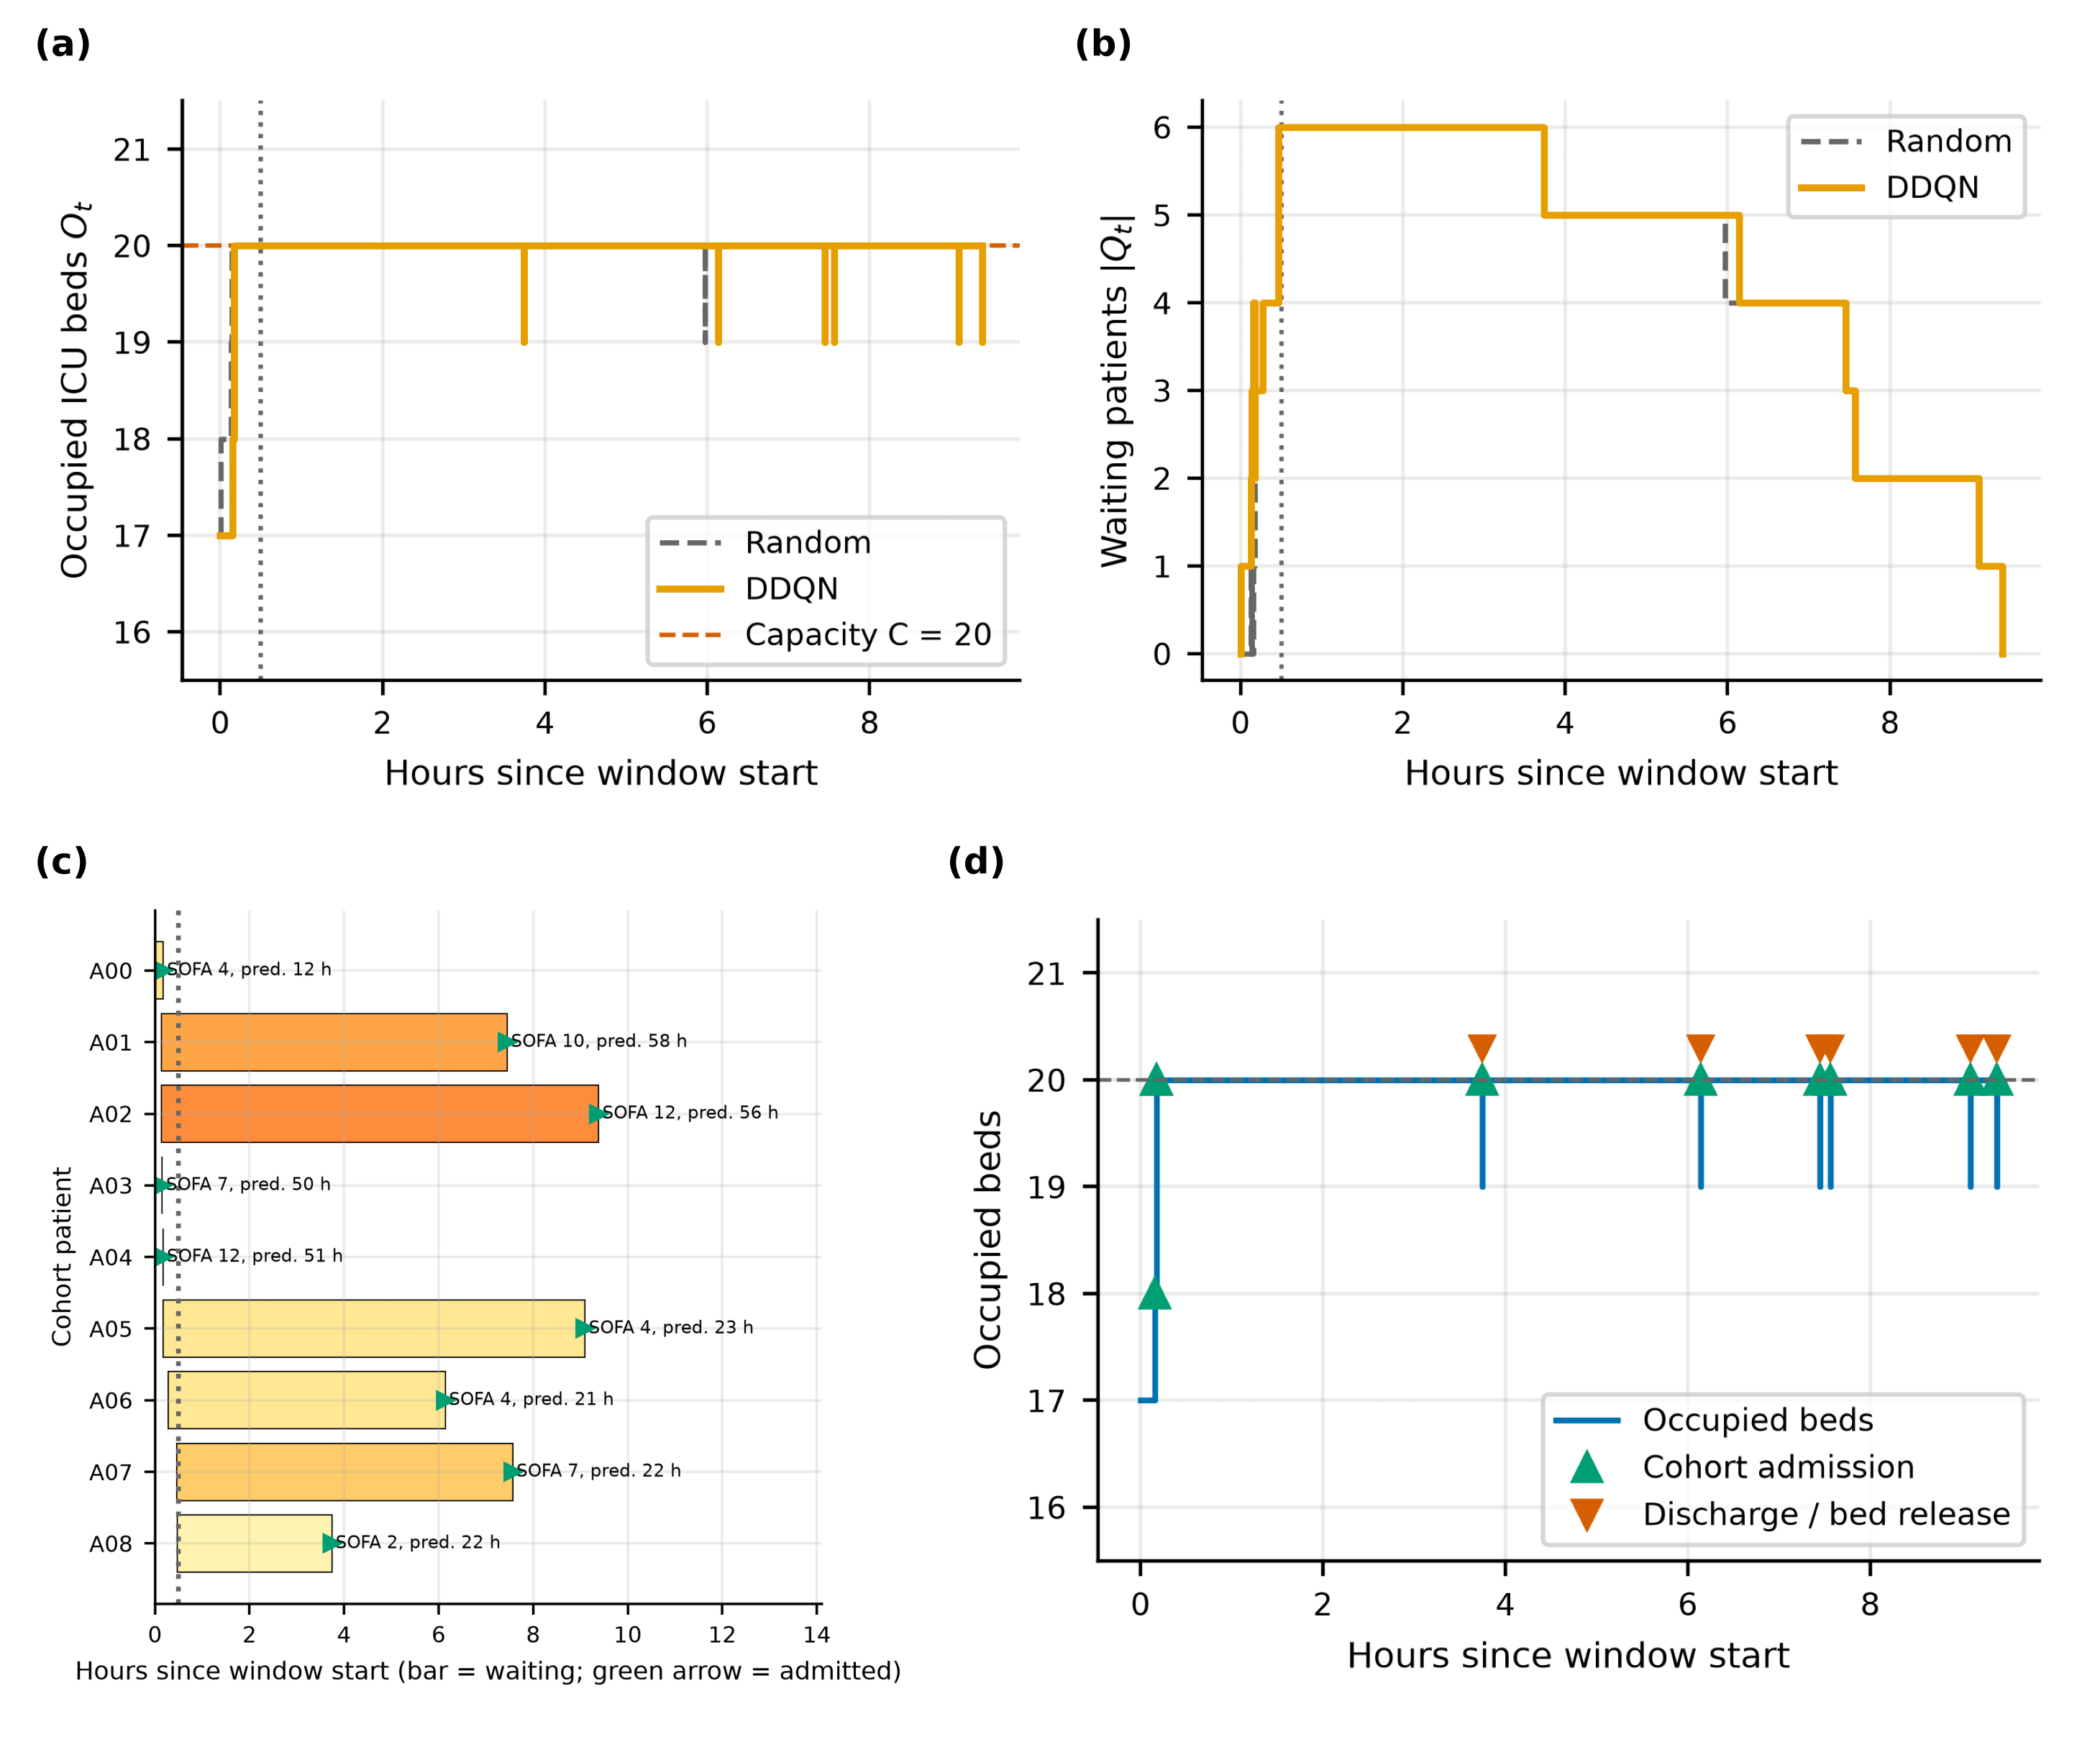
\includegraphics[width=0.82\textwidth]{agent_snapshots.png}
  \caption{DDQN in test episode 21: (a) ICU occupancy and (b) queue size for DDQN and Random (capacity is never exceeded); (c) DDQN admission decisions, bar = waiting time coloured by SOFA, arrow = admission; (d) bed releases followed by admissions.}
  \label{fig:snap}
\end{figure*}


\subsection*{2) Selecting the best algorithm}
Table~\ref{tab:select} lists the quantitative criteria. On \emph{robustness across seeds}, DDQN has the smallest spread of test total wait (SD 0.63) and all five of its seeds beat Random (56.95--58.52 vs.\ Random's best seed 59.99). DQN is similar (SD 0.71, all seeds better than Random). PPO is not robust (SD 6.15, two of five seeds worse than Random). On \emph{convergence efficiency}, DDQN meets the criterion earliest (500 episodes), DQN later (1{,}667) and PPO latest (2{,}133). Few seeds meet the criterion at all, so this ranking is weak. On \emph{computational cost}, PPO is about 4.4$\times$ cheaper ($312\pm56$ s per run vs.\ $1{,}338\pm53$ s for DQN and $1{,}371\pm87$ s for DDQN). PPO makes one batched update per 32 episodes, while the DQN variants update after every transition. On \emph{test performance}, DQN's mean total wait is 0.39 patient-hours lower than DDQN's, but the paired difference is not significant (95\,\% CI [$-0.02,0.82$]).

We therefore select \textbf{DDQN}. It is best on the two criteria the protocol prescribes, convergence efficiency and robustness, and is statistically tied with DQN on test performance. PPO is ruled out by its seed instability despite its speed. A plausible explanation is that Double Q-learning's decoupled selection and evaluation reduce the overestimation that a max over noisy, high-variance targets produces. The PPO failures, in turn, look like early collapse onto a poor deterministic ordering, from which its on-policy updates did not recover. We did not run a systematic hyperparameter search, so these explanations are hypotheses. The ranking also differs from run (iii) on the single 10:00 window, where PPO was best. The choice of algorithm is therefore not stable across scenario designs.

\subsection*{3) Reward comparison for the selected algorithm}
DDQN was retrained with Reward~2 ($\alpha=\beta=1$) using the same five seeds and budget. Both sets of policies were evaluated on the same 200 test episodes (Table~\ref{tab:reward}, Fig.~\ref{fig:reward}). Reward~2 shortens the mean wait of high-SOFA patients from 6.43 to 5.30 h. The paired difference is $-1.13$ h [$-1.31,-0.95$], a 17.6\,\% reduction. The price is a small increase in total waiting of $+1.14$ patient-hours [$0.50,1.89$] (+2.0\,\%) and of the maximum wait (8.61 to 8.75 h). The severity-weighted cost, computed post hoc with arrival SOFA, does not change significantly ($+0.39$ [$-0.33,1.18$]). Each policy is slightly better on the return of its own training reward, which is the expected sign: $-2.89$ vs.\ $-2.94$ under $R_1$, and $-5.43$ vs.\ $-5.45$ under $R_2$. Both rewards still beat Random on total waiting. Reward~2 also beats Random on severity-weighted cost (70.2 vs.\ 72.2), while keeping high-SOFA waiting near Random's level (5.30 vs.\ 5.42 h) rather than letting it grow as under Reward~1.

\textbf{Sensitivity.} Three-seed DDQN runs with other coefficients (Fig.~\ref{fig:sens}) trace the trade-off between total waiting (patient-hours) and high-SOFA waiting. With $(\alpha,\beta)=(0,1)$, where only waiting time matters, the policy reaches 56.0 and 6.89 h. With $(0.25,1)$ it reaches 56.6 and 6.23 h, and the default $(1,1)$ reaches 58.9 and 5.30 h. Severity-dominated weights $(1,0.25)$ and $(1,0)$ give 67.5/3.30 h and 69.6/3.11 h, close to the SOFA-first heuristic. The coefficient $\alpha$ therefore acts as a dial between aggregate delay and fast admission of severe patients. Even the strongest severity weighting shortens high-SOFA waits by only about 2.3 h, at the cost of about 12 additional patient-hours in total.

\textbf{Which reward wins?} Neither reward dominates. Reward~1 is better on aggregate delay and on the maximum wait. Reward~2 trades about 2\,\% more total waiting for about 18\,\% shorter waits of the severest patients, which a clinical team may well prefer. The choice is a value judgement and not an empirical one, and we report both.

\begin{table}[!t]
  \caption{DDQN trained with Reward~1 vs.\ Reward~2, same 200 test episodes (mean $\pm$ SD over 5 seeds).}
  \label{tab:reward}
  \centering
  \footnotesize
  \setlength{\tabcolsep}{4pt}
  \begin{tabular}{lcc}
    \toprule
    \textbf{Metric} & \textbf{DDQN, Reward~1} & \textbf{DDQN, Reward~2} \\
    \midrule
    Total wait (patient-h) & 57.74 $\pm$ 0.63 & 58.87 $\pm$ 1.40 \\
    Mean wait (h) & 4.87 $\pm$ 0.11 & 4.90 $\pm$ 0.15 \\
    Max wait (h) & 8.61 $\pm$ 0.24 & 8.75 $\pm$ 0.37 \\
    High-SOFA wait (h) & 6.43 $\pm$ 0.42 & 5.30 $\pm$ 0.65 \\
    Severity-wtd cost & 69.84 $\pm$ 0.40 & 70.23 $\pm$ 0.84 \\
    Deterioration events & 6.60 & 6.51 \\
    Completion / unresolved & 100\% / 0 & 100\% / 0 \\
    Utilisation & 0.974 & 0.978 \\
    Return under $R_1$ & $-2.89$ & $-2.94$ \\
    Return under $R_2$ & $-5.45$ & $-5.43$ \\
    \bottomrule
  \end{tabular}
\end{table}

\begin{figure*}[!t]
  \centering
  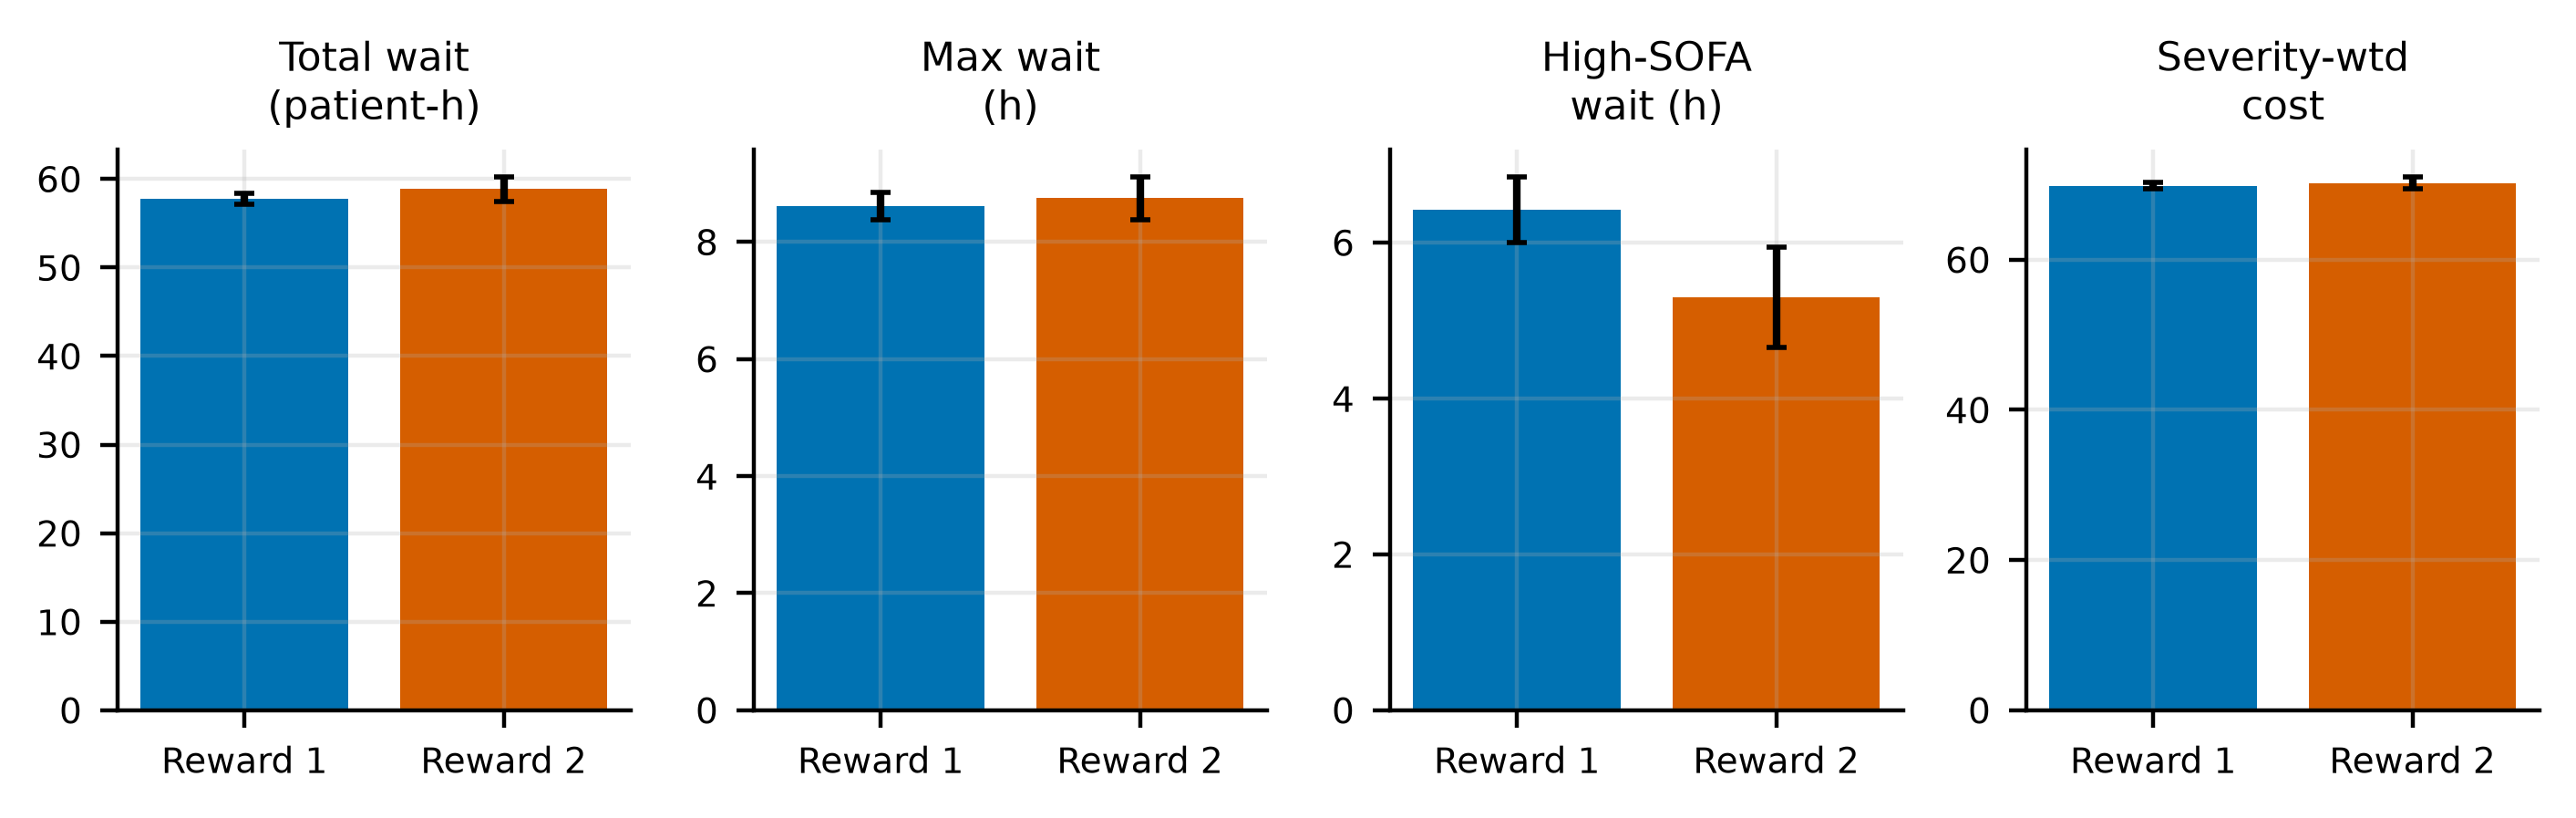
\includegraphics[width=0.9\textwidth]{reward_comparison.png}
  \caption{DDQN trained with Reward~1 versus Reward~2 on identical test episodes (error bars: SD across seeds).}
  \label{fig:reward}
\end{figure*}
\begin{figure}[!t]
  \centering
  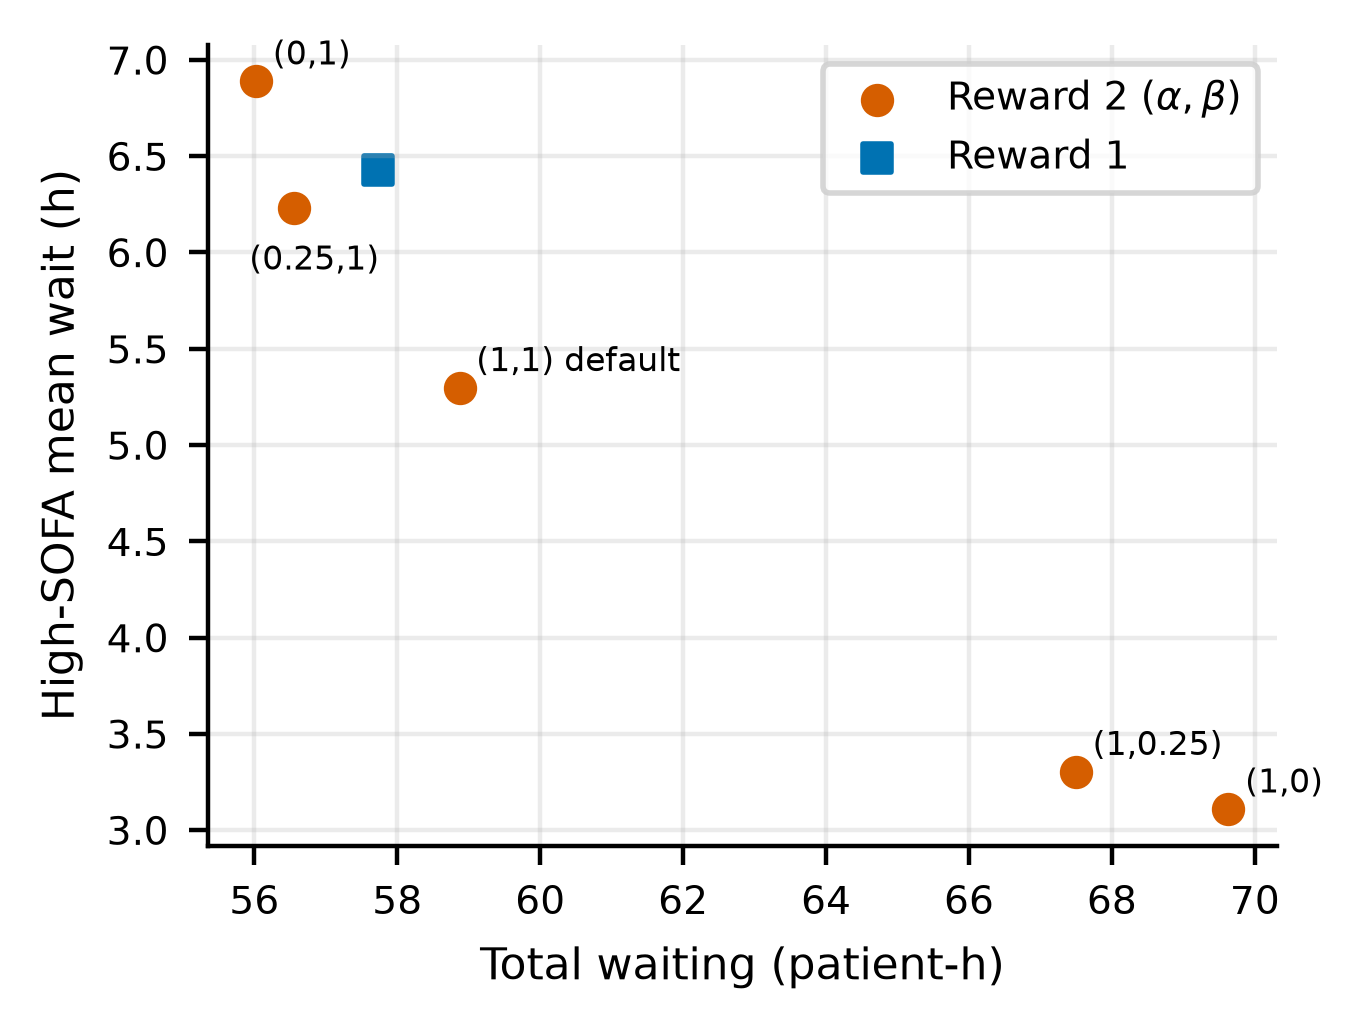
\includegraphics[width=0.95\columnwidth]{reward_sensitivity.png}
  \caption{Sensitivity of DDQN to the Reward~2 coefficients $(\alpha,\beta)$: total waiting vs.\ high-SOFA waiting (mean over seeds).}
  \label{fig:sens}
\end{figure}

\section{Conclusion}
\textbf{Findings.} We simulated a single ICU in which every 30-minute arrival window of the day forms an episode. DQN, DDQN and PPO all reduced total waiting relative to random allocation (DQN $-5.1$\,\%, DDQN $-4.4$\,\%, PPO $-1.7$\,\%), with no capacity violations. DDQN was selected as the best algorithm on convergence efficiency and seed robustness, and it is statistically tied with DQN on test performance. PPO was the cheapest to train but unstable across seeds. No learner matched a simple shortest-predicted-stay heuristic, and the gains are modest. Reward~2 offers a clear and tunable priority for severe patients: high-SOFA waiting falls from 6.4 to 5.3 h at the cost of 2\,\% more total waiting. Neither reward is better on every metric, so the choice depends on whether aggregate delay or waits of the severest patients matter more.

\textbf{Assumptions.} Synthetic latent-severity data; a sinusoidal time-of-day demand pattern; each window drawn independently with its own census; stays that depend on severity and are partly predictable; independent deterioration hazards; no pre-emption; capacity the only constraint; instantaneous admission; congestion levels chosen by us.

\textbf{Limitations.} The data are synthetic, and the stay predictor overstates waiting patients' stays about 3.2-fold (rank-preserving; see Section~\ref{sec:data}), so nothing here is a clinically validated model or evidence of patient benefit. The simulator was made more learnable during development, as disclosed above, so the effect sizes describe this simulator only, and the algorithm ranking changed between scenario designs. Consecutive windows are not linked: the census of one window does not carry over to the next. Only five seeds and one network size were studied, and no systematic hyperparameter search was run. Ordering effects are small relative to the variance between episodes. Deterioration predictions on training episodes are in-sample after a deterioration event. Mortality, transfers, staffing and equipment are not modelled. Finally, test episodes come from the same synthetic distribution as the training episodes.

\textbf{Future work.} Chain consecutive windows so that each census follows from the previous allocations. Replace the synthetic records with credentialed MIMIC-IV or other real data, which the file layout already supports. Validate the predictors of stay and deterioration against real outcomes. Calibrate the diurnal arrival pattern and congestion levels to a real hospital. Run hyperparameter searches with more seeds, and compare against queueing-theory policies. Study off-policy evaluation and obtain clinical review before any practical consideration.

\textbf{Contributions of each contributor.} [To be completed by the authors: names and responsibilities were not supplied and have not been invented.]

\FloatBarrier
% ---- References (stored separately in ref.bib) ----
\bibliographystyle{ieeetr}
\bibliography{ref}

\onecolumn
\section*{Appendix}
\subsection{Code}
The complete implementation is in the project repository (\texttt{src/}); only key excerpts are shown.

\begin{lstlisting}[language=Python, caption=SOFA components from raw variables (sofa\_calculator.py)]
def resp_score(pf, vent):
    s = np.zeros(pf.shape, int)
    s = np.where(pf < 400, 1, s); s = np.where(pf < 300, 2, s)
    s = np.where((pf < 200) & vent, 3, s)
    s = np.where((pf < 100) & vent, 4, s)
    return s
def coag_score(plt):  # platelets 10^3/uL
    return np.select([plt<20, plt<50, plt<100, plt<150], [4,3,2,1], 0)
def liver_score(b):   # bilirubin mg/dL
    return np.select([b>=12, b>=6, b>=2, b>=1.2], [4,3,2,1], 0)
def cv_score(map_, drug, dose):
    s = np.where(map_ < 70, 1, 0)
    s = np.where(drug == 1, np.select([dose>15, dose>5], [4,3], 2), s)
    s = np.where(drug == 2, np.where(dose > 0.1, 4, 3), s)
    return s
def cns_score(gcs):
    return np.select([gcs<6, gcs<10, gcs<13, gcs<15], [4,3,2,1], 0)
def renal_score(creat, uo):  # uo mL/day
    sc = np.select([creat>=5, creat>=3.5, creat>=2, creat>=1.2], [4,3,2,1], 0)
    su = np.select([uo < 200, uo < 500], [4, 3], 0)
    return np.maximum(sc, su)
# total = sum of the six components (0..24)
\end{lstlisting}

\begin{lstlisting}[caption=Synthetic episode generation (pseudocode)]
for each episode e (seeded by [seed, e]):
    scenario ~ {low, medium, high};  free_beds ~ U(range)
    n_occ = C - free_beds;  n_arr = max(1, Poisson(mean))
    arrival times: rejection sampling, intensity ~ 1 + 0.4 t/T on [0, 30 min), sorted
    for each patient: z ~ Beta(2,3); noise ~ N(0,1)^14; u ~ U(0,1)^3; age
        raw = f(z, age, noise, u)          # deterministic map
        SOFA = sum of six component scores (raw)
        L = lognormal stay; occupants: elapsed = U(0.1,0.9) * L, remaining >= 0.5 h
        hazard = exp(log 0.03 + 2.2 z + ... + frailty)
        deterioration budgets E_k ~ Exp(1), jumps dz_k ~ U(0.08, 0.18)
fit predictors on train episodes only; out-of-fold predictions for train rows
write observable files (snapshots, arrivals, census, predictions) and hidden files
\end{lstlisting}

\begin{lstlisting}[caption=Event-driven simulation core (pseudocode)]
reset(e): t = 0; push discharge of each occupant; push arrival of each cohort
          patient; push window-end at 0.5 h; advance to the first decision
advance(): loop
    if window closed and queue empty and all arrived: done
    if beds > 0 and queue nonempty and not just-STOPped: return (decision epoch)
    t_next = earliest event; if t_next > horizon: charge to horizon, unresolved
        patients get penalty, done
    cost += interval_cost(queue, t_next - t); occupancy_area += beds_used*(dt)
    process all events at t_next in order: discharge < arrival < deterioration < end
step(a): ADMIT(i): status=ICU; schedule discharge at t + actual_stay; if more beds
         and queue: stay in same epoch (dt = 0) else advance()
         STOP: advance() to the next event; reward = -cost * scale
\end{lstlisting}

\begin{lstlisting}[language=Python, caption=Reward integration (reward\_functions.py)]
def clipped_wait_integral(w0, dt, wref):
    tau = np.maximum(wref - w0, 0.0)
    ramp_t = np.minimum(dt, tau)
    ramp = (w0 * ramp_t + 0.5 * ramp_t**2) / wref
    return ramp + (dt - ramp_t)

def interval_cost(kind, sofa, wait0, dt, p):
    if kind == "r1": return len(sofa) * dt
    S = np.asarray(sofa) / 24.0
    return p["alpha"]*S.sum()*dt + p["beta"]*clipped_wait_integral(wait0, dt, p["wref"]).sum()
\end{lstlisting}

\noindent\begin{minipage}{\linewidth}
\begin{lstlisting}[caption=DQN / DDQN and PPO updates (pseudocode)]
DQN/DDQN: for each transition (s,a,r,s',done,dt) stored in replay:
    disc = gamma ** (dt / tau0)
    a* = argmax_valid Q_online(s')         # DDQN;  DQN: max_valid Q_target(s')
    y  = r + (1-done) * disc * Q_target(s', a*)
    minimise Huber(Q_online(s,a) - y); hard-update target every 250 updates
PPO: collect 32 episodes with the masked softmax policy
    delta_t = r_t + g_t V(s_{t+1}) - V(s_t),  g_t = gamma ** (dt_t / tau0)
    A_t = delta_t + g_t * lambda * A_{t+1};  normalise A
    4 epochs of clipped surrogate + 0.5 value loss - 0.01 entropy
\end{lstlisting}
\end{minipage}

\subsection{Anything else}
\begin{figure}[!ht]
  \centering
  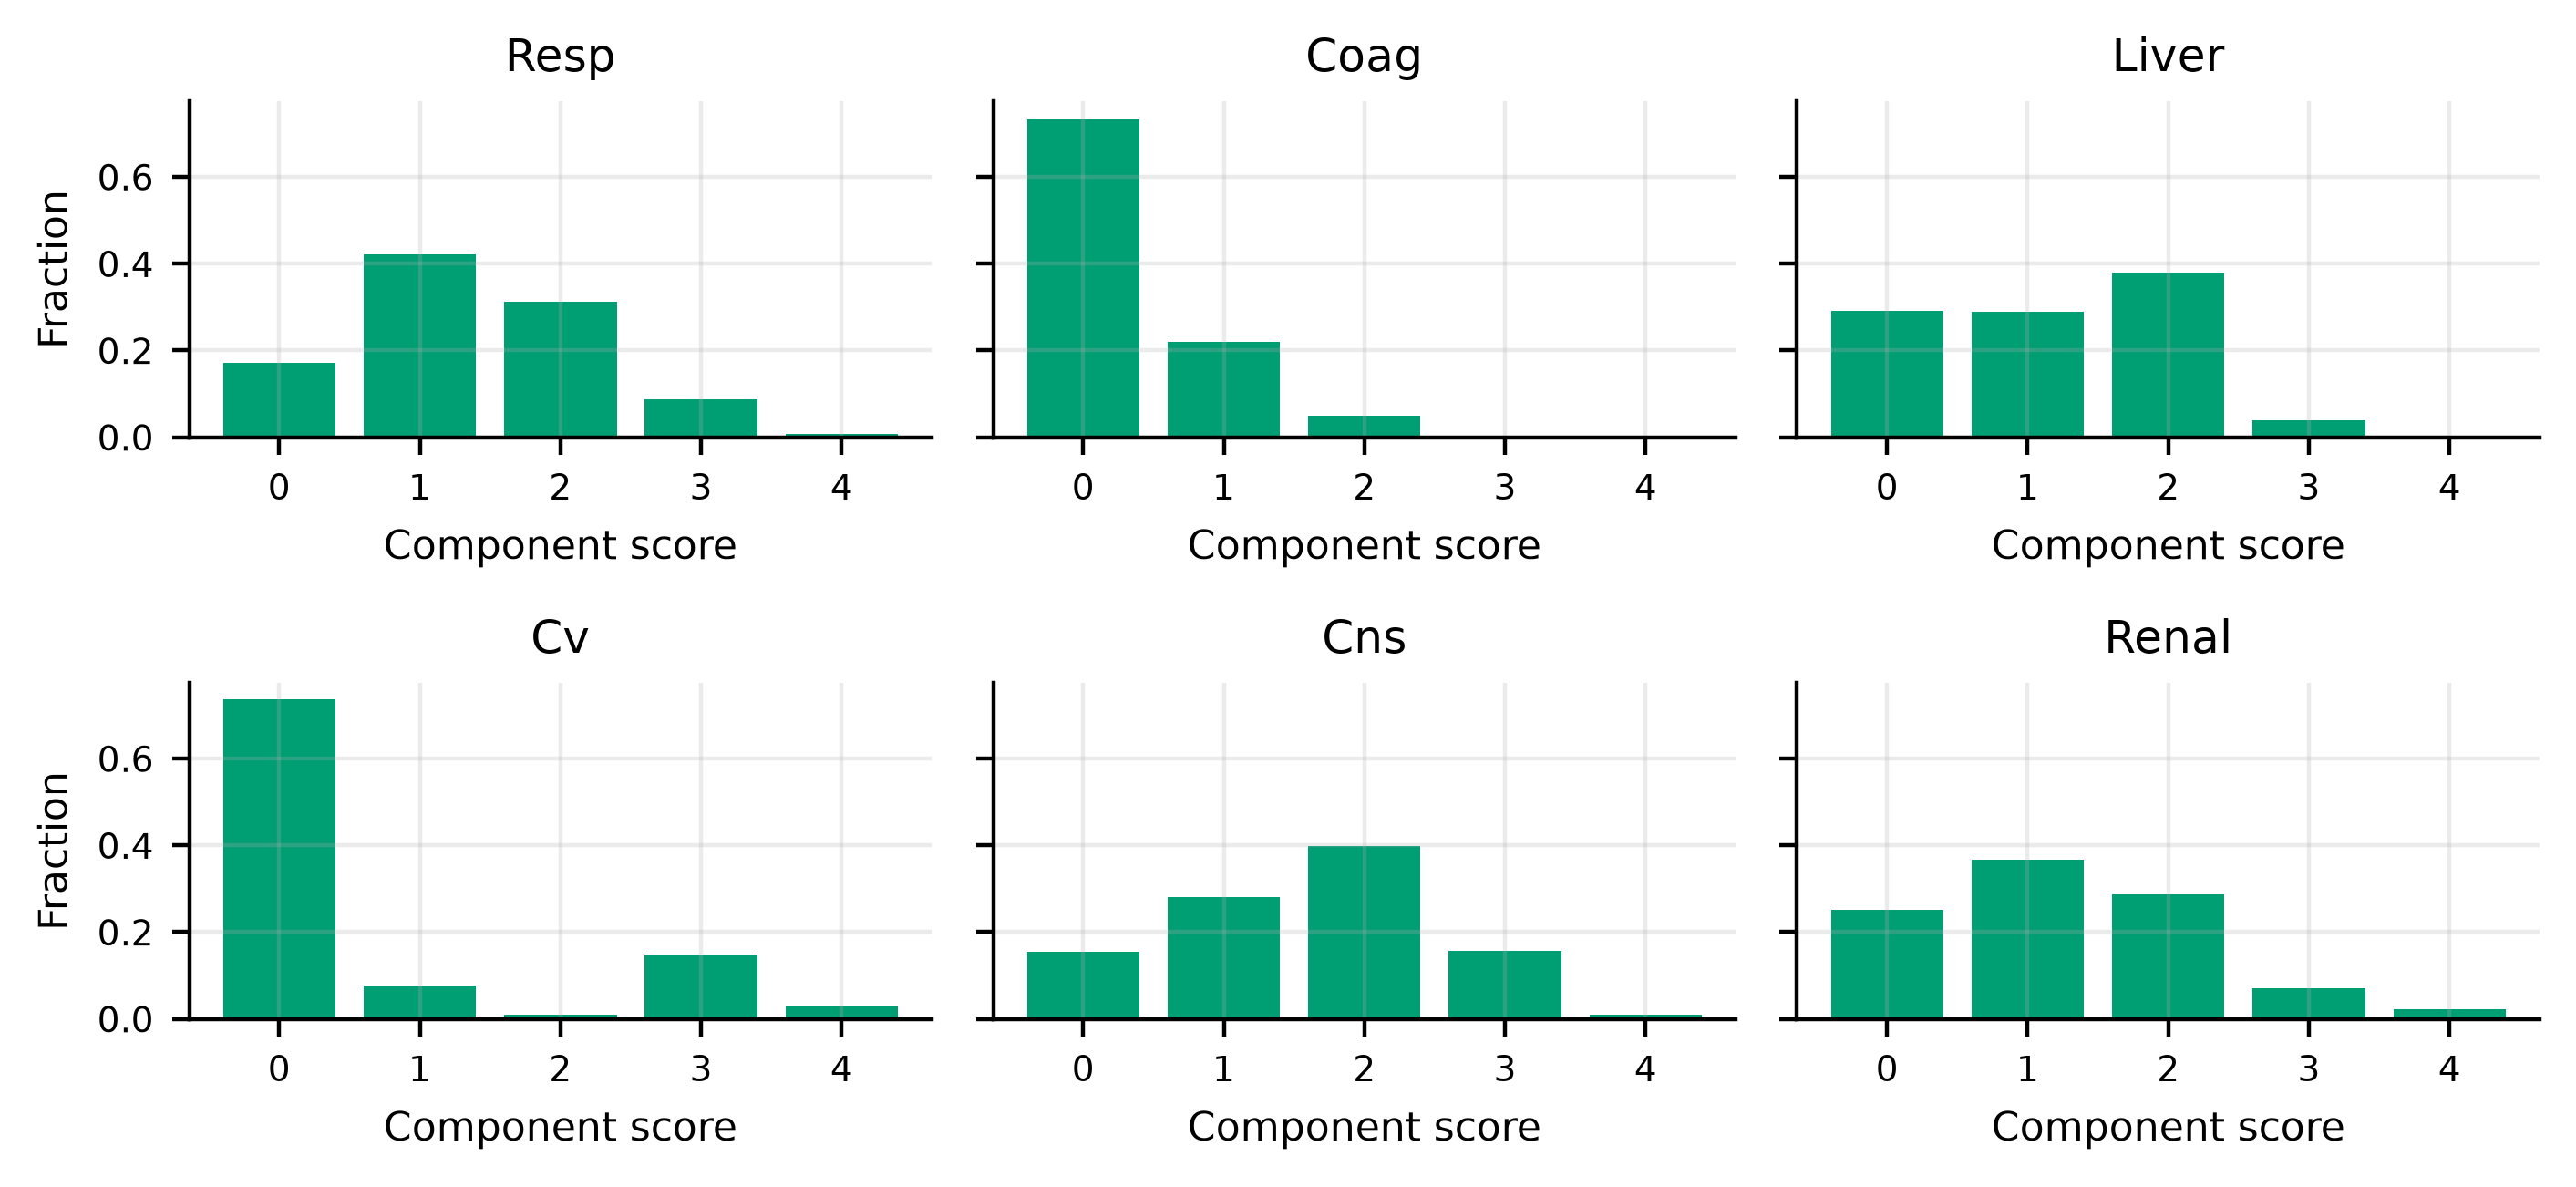
\includegraphics[width=0.8\textwidth]{sofa_components.png}
  \caption{Distribution of the six SOFA component scores (all synthetic patients).}
  \label{fig:comp}
\end{figure}
\textbf{Reproducibility.} The commands to regenerate the data, tests, training runs, evaluations and figures are in \texttt{README.md}; configuration is in \texttt{config.yaml}. Test coverage: 19 automated test functions cover capacity, window membership, coverage of all 48 daily windows, hidden information, event ordering, SOFA thresholds, reward integrals, masking, permutation equivariance and seed reproducibility.

\textbf{Metrics.} Total waiting is the sum of cohort waiting times (patient-hours); a patient still waiting at the horizon contributes the censored time $t_{horizon}-t^{request}$. Severity-weighted waiting cost is evaluated post hoc as $\sum_i(\alpha\mathrm{SOFA}_i/24+\beta\min(W_i/W_{ref},1))W_i$ with arrival SOFA. ICU utilisation is time-weighted occupied beds over capacity from the window start to the last cohort admission, and is descriptive only.
\end{document}
